\documentclass[../main.tex]{subfiles}
 
\begin{document}

\chapter{Results}\label{sec: Results}

Natural units ($\hbar=c=e=m_e=1$) were used to obtain all the results listed in this chapter.

\section{Optimization}

Here we look at the effect that various optimizations had on the computation time of our program. The optimization to the simulation itself gave a total speed-up factor of $31.246$ for the tested system, while running the program in parallel on $4$ processors gave an additional speed-up factor of around $3.6$.

\subsection{Storing Reused Data and Optmizing Hermite Polynomials}

For the following optimization results we used a system of two particles in a two-dimensional double harmonic oscillator well as reference system. For the results in Table \ref{tab: OptimizationExpansion} we used $465$ basis functions. From the table we see that including the "-ffast-math" compiler flag gives a decent speed up, but the storing of the Slater related matrices and the efficient computation of Hermite polynomials are the most important optimizations in this case. We also see that the "-ffast-math" flag is much more important when we include the Hermite optimization described in Section \ref{sec:Optimizing Hermite}. In this case the storing of the relative distances and the Jastrow related matrices, provide seemingly no speed up. This makes sense since these optimizations scale well with the number of particles used, and therefore become important for large numbers of particles. In our case we only have two particles so the effect of these optimizations is negligible. The optimization of Hermite polynomial calculation obviously scales with the number of Hermite polynomials we need. The number of Hermite polynomials we need scales with the number of basis functions we use, and in our case we use $465$ basis functions, which means we need the first $30$ Hermite polynomials, each of which has to be calculated many times for various positions of particles. The efficiency gain from storing the Slater related matrices also scales with the number of basis functions. This is because these matrices store the single particle wave functions and their derivatives. These single particle wave functions are calculated by a loop over the number of basis functions, so if we avoid recalculating them unnecessarily, we reduce the number of basis function loops, which of course is more important if we use a lot of basis functions.

\begin{table}[!ht]
  \centering
  \begin{tabular}{ | c | c | c | c |}
    \hline
    Optmizations & Avg. Time [s] & Speed Up & Total Speed Up\\*
    \hline
    B & 122.173 & 1.000 & 1.000\\*
    \hline
    B F & 104.244 & 1.172 & 1.172\\*
    \hline
    B F D & 104.296 & 1.000 & 1.171\\*
    \hline
    B F D S & 16.8304 & 6.197 & 7.259\\*
    \hline
    B F D S J & 16.8524 & 0.999 & 7.250\\*
    \hline
    B F D S J H & 3.91007 & 4.310 & 31.246\\*
    \hline
    B D S J H & 30.7192 & 0.127 & 4.017\\*
    \hline
  \end{tabular}
  \caption{Optimization results for two particles in a two-dimensional double harmonic oscillator well. The number of basis functions used was $465$. The letter B stands for base i.e. the program before doing optimizations. The letter F is for using the "-ffast-math" compiler flag, D is for storing the distance matrix, S is for storing the Slater related matrices, J is for storing the Jastrow related matrices, and H is for optimal computation of Hermite polynomials. The "Avg. Time" column is the average time over five runs, the "Speed Up" column lists the speed up factor relative to the row above, and the "Total Speed Up" column lists the speed up factor relative to the first row. Optimizations D and J have seemingly no effect on the run-time, because they scale with the number of particles and we only use two particles in this case. The gain from using the F optimization is much greater when we also use the H optimization. This is apparent by comparing the first two rows with the last two rows. The S and H optimizations provide the most speed up for this system.}
  \label{tab: OptimizationExpansion}
\end{table}

%\begin{table}[!ht]
%  \centering
%  \begin{tabular}{ | c | c | c | c | c | c | c | c | c |}
%    \hline
%    Optmizations & Run 1 & Run 2 & Run 3 & Run 4 & Run 5 & Avg. & Speed Up & Total\\*
%    \hline
%    B & 122.074 & 122.730 & 122.223 & 122.006 & 121.834 & 122.173 & 1.000 & 1.000\\*
%    \hline
%    B F & 104.236 & 104.029 & 103.951 & 104.515 & 104.489 & 104.244 & 1.172 & 1.172\\*
%    \hline
%    B F D & 103.960 & 104.523 & 104.207 & 104.359 & 104.429 & 104.296 & 1.000 & 1.171\\*
%    \hline
%    B F D S & 16.8619 & 16.6298 & 16.9949 & 16.8100 & 16.8552 & 16.8304 & 6.197 & 7.259\\*
%    \hline
%    B F D S J & 16.8360 & 16.9138 & 17.0127 & 16.8403 & 16.6593 & 16.8524 & 0.999 & 7.250\\*
%    \hline
%    B F D S J H & 3.99471 & 3.87888 & 3.89648 & 3.74037 & 4.03992 & 3.91007 & 4.310 & 31.246\\*
%    \hline
%    B D S J H & 30.8744 & 30.7226 & 30.8116 & 30.7741 & 30.4132 & 30.7192 & 0.127 & 4.017\\*
%    \hline
%  \end{tabular}
%  \caption{}
%  \label{tab: OptimizationExpansion}
%\end{table}

In order to see that storing the distances and the Jastrow related matrices do actually contribute to the optimization, we will look at a different system. We now look at a system of $24$ particles in a two-dimensional double harmonic oscillator well. However, we now approximate the single particle wave functions with super positions of two harmonic oscillator functions, similarly to what was done in Chapter 5.1.3 and 5.2.3 of Ref. \cite{Jorgen}. This means that the number of Hermite calculations needed is significantly reduced, and the effect of storing the distances and the Jastrow related matrices should stand out due to the increased number of particles. Note that this way of calculating the single particle wave functions is not the focus of this thesis, but it has been implemented in order to compare the results of the two methods. In this case we use this method in order to simulate $24$ particles with reasonably short run times, as this method is generally faster especially for large number of particles. The benefit of storing the distances and the Jastrow related matrices should be similar for both methods, since the difference between them is how the single particle wave functions are calculated, and these single particle wave functions do not depend on the Jastrow factor or the distances between particles. The optimization results for this system are listed in Table \ref{tab: OptimizationSupPos}. As expected the importance of storing the distances and the Jastrow related matrices has gone up. The storing of distances provide a decent speed up, while the storing of the Jastrow related matrices is in this case the most important optimization. The storing of the Slater related matrices is not quite as important as it was in Table \ref{tab: OptimizationExpansion}, but it still provides a pretty good speed up. The effect of using the "-ffast-math" flag is much smaller in this case, and the effect of calculating Hermite polynomials is negligible. This method needs a lot less Hermite polynomial calculations, since there is no loop over basis functions when calculating the single particle wave functions. However, the number of Hermite polynomial calculations does scale with the number of particles, and the recursive method becomes slow for large numbers of particles, so for systems with even more particles the Hermite optimization should become significant for this method as well.

\begin{table}[!ht]
  \centering
  \begin{tabular}{| c | c | c | c |}
    \hline
    Optmizations & Avg. Time [s] & Speed Up & Total Speed Up\\*
    \hline
    B & 103.576 & 1.000 & 1.000\\*
    \hline
    B F & 101.766 & 1.018 & 1.018\\*
    \hline
    B F D & 92.2338 & 1.103 & 1.123\\*
    \hline
    B F D S & 54.7138 & 1.686 & 1.893\\*
    \hline
    B F D S J & 10.7135 & 5.107 & 9.668\\*
    \hline
    B F D S J H & 10.6977 & 1.001 & 9.682\\*
    \hline
    B D S J H & 10.8811 & 0.983 & 9.519\\*
    \hline
  \end{tabular}
  \caption{Optimization results for $24$ particles in a two-dimensional double harmonic oscillator well. The letter B stands for base i.e. the program before doing optimizations. The letter F is for using the "-ffast-math" compiler flag, D is for storing the distance matrix, S is for storing the Slater related matrices, J is for storing the Jastrow related matrices, and H is for optimal computation of Hermite polynomials. The "Avg. Time" column is the average time over five runs, the "Speed Up" column lists the speed up factor relative to the row above, and the "Total Speed Up" column lists the speed up factor relative to the first row. The single particle wave functions were approximated by a super position of two harmonic oscillator functions instead of the method regularly used in this thesis. The method used here involves less Hermite polynomial calculations, and as a result, optimizing the calculation of Hermite polynomials is less important. The benefit of optimizations D and J should be similar between the methods, and now that the number of particles is increased the effect of these optimizations is also increased compared to Table \ref{tab: OptimizationExpansion}. Optimazation D now provides a decent speed up, while optimization J provides the majority of the total speed up. Optimization S also provides a good speed up, but it is not as significant as it was in Table \ref{tab: OptimizationExpansion}.}
  \label{tab: OptimizationSupPos}
\end{table}

%\begin{table}[!ht]
%  \centering
%  \begin{tabular}{ | c | c | c | c | c | c | c | c | c |}
%    \hline
%    Optmizations & Run 1 & Run 2 & Run 3 & Run 4 & Run 5 & Avg. & Speed Up & Total\\*
%    \hline
%    B & 103.804 & 103.122 & 103.119 & 104.314 & 103.523 & 103.576 & 1.000 & 1.000\\*
%    \hline
%    B F & 101.842 & 100.080 & 99.9448 & 100.403 & 106.561 & 101.766 & 1.018 & 1.018\\*
%    \hline
%    B F D & 91.8727 & 91.5986 & 94.2381 & 91.8457 & 91.6137 & 92.2338 & 1.103 & 1.123\\*
%    \hline
%    B F D S & 54.4560 & 55.5666 & 54.3716 & 54.3464 & 54.8286 & 54.7138 & 1.686 & 1.893\\*
%    \hline
%    B F D S J & 10.6361 & 10.9981 & 10.6575 & 10.7927 & 10.4832 & 10.7135 & 5.107 & 9.668\\*
%    \hline
%    B F D S J H & 10.5354 & 10.7410 & 10.9612 & 10.7303 & 10.5204 & 10.6977 & 1.001 & 9.682\\*
%    \hline
%    B D S J H & 10.8578 & 10.8000 & 10.8382 & 10.8467 & 11.0629 & 10.8811 & 0.983 & 9.519\\*
%    \hline
%  \end{tabular}
%  \caption{}
%  \label{tab: OptimizationSupPos}
%\end{table}

\subsection{Parallelization}

As discussed in Section \ref{sec:Parallel}, the variational Monte Carlo (VMC) simulation can be parallelized without mid-simulation communication between the processors. Therefore we can expect near linear scaling, so doubling the number of processors should about halve the run time. In Table \ref{tab: Parallel1} we have listed average run times for a system of two particles in a two-dimensional double harmonic oscillator well, when using $1275$ basis functions and $1$, $2$ and $4$ processors. From the table we see that the speed up is close to what we expect, but not quite. 

\begin{table}[!ht]
  \centering
  \begin{tabular}{| c | c | c | c |}
    \hline
    Processors & Avg. Time [s] & Speed Up & Total Speed Up\\*
    \hline
    1 & 36.9145 & 1.0000 & 1.0000\\*
    \hline
    2 & 19.1713 & 1.9255 & 1.9255\\*
    \hline
    4 & 10.3109 & 1.8593 & 3.5801\\*
    \hline
  \end{tabular}
  \caption{Parallelization results for two particles in a two-dimensional double harmonic oscillator well. The number of basis functions used was $1275$. The "Avg. Time" column is the average time over five runs, the "Speed Up" column lists the speed up factor relative to the row above, and the "Total Speed Up" column lists the speed up factor relative to the first row. We see that doubling the number of processors gives a speed up factor close to $2$, but it is still somewhat off, especially when going from $2$ to $4$ processors.}
  \label{tab: Parallel1}
\end{table}

A possible reason for why the results in Table \ref{tab: Parallel1} were somewhat different than expected could be that the run times were so short that the parallel overhead\footnote{Parallel overhead is the amount of time required to coordinate parallel tasks, as opposed to doing useful work. This can include factors such as: start-up time, synchronizations, data communications, software overhead imposed by libraries, operating system, etc., and termination time.\cite{Blaise}} was responsible for a significant fraction of the run time. If this is the case, doing the same test for a system that requires more CPU time, should provide results closer to the near linear scaling we expect. We increase the number of particles to $4$, and the run times for this system are listed in Table \ref{tab: Parallel2}. We end up with run times which are about three times as long as for the previous system, and as expected the speed up from parallelization is indeed somewhat greater for this system than for the two-particle system.

\begin{table}[!ht]
  \centering
  \begin{tabular}{| c | c | c | c |}
    \hline
    Processors & Avg. Time [s] & Speed Up & Total Speed Up\\*
    \hline
    1 & 107.468 & 1.0000 & 1.0000\\*
    \hline
    2 & 55.4418 & 1.9384 & 1.9384\\*
    \hline
    4 & 29.4316 & 1.8838 & 3.6514\\*
    \hline
  \end{tabular}
  \caption{Parallelization results for $4$ particles in a two-dimensional double harmonic oscillator well. The number of basis functions used was $1275$. The "Avg. Time" column is the average time over five runs, the "Speed Up" column lists the speed up factor relative to the row above, and the "Total Speed Up" column lists the speed up factor relative to the first row. We see that doubling the number of processors gives a speed up factor close to $2$, and the speed up factor are closer to $2$ in this case than they were in Table \ref{tab: Parallel1}. This is likely due to the generally longer run times for this system compared to the two-particle system. Since the run time is longer, the overhead is a smaller percentage of the total run time, which means it has less of an effect on the speed up factors.}
  \label{tab: Parallel2}
\end{table}

\section{Single Harmonic Oscillator Well}

In this section we look at the energy and one-body density of systems of particles in a single harmonic oscillator potential well, both in two and three dimensions.

\subsection{Ground State Energies}\label{sec: SHO GSE}

Here we look at the ground state energies for systems with various $\omega$ and number of particles. The ground state energies are calculated with the single particle wave functions being approximated by expansion in a single harmonic oscillator basis, and also by using harmonic oscillator single particle wave functions directly. Since the wave functions we are trying to approximate and the basis functions we use are of the same type (single harmonic oscillator) we should expect the two methods to yield the exact same results using a small amount of basis functions, just as we saw for the non-interacting case in Section \ref{sec:testSHO}. It turns out that we do not get the exact same results for the interacting case, however the same results are achieved if the variational parameter $\alpha$ is kept constant at $\alpha = 1$, while the other variational parameter $\beta$ is varied as usual. This indicates that there is an $\alpha$ dependence in the coefficients used in the basis function expansion, which our method fails to include. This $\alpha$ dependence could be included by doing a Hartree-Fock calculation on the coefficients, and this would be the next step in improving the method, but has not been done in this thesis.

\subsubsection{Two Dimensions}

The ground state energies for the two-dimensional case are listed in Table \ref{tab: EnergiesSHO2D}. The energies $E_\textrm{coeff}$ are the results when the single particle wave functions are approximated by expansion in a single harmonic oscillator basis, while $E_\textrm{reg}$ are the results when using harmonic oscillator single particle wave functions directly. We see from the table that $E_\textrm{coeff}$ and $E_\textrm{reg}$ are similar, especially for small numbers of particles $N$, but they are not exactly equal. Some further calculations not included here, revealed that the exact same energies where achieved if $\alpha$ was held constant at $\alpha = 1$, and $\beta$ was treated as the only variational parameter. This indicates that there is an $\alpha$ dependence in the coefficients used in the basis function expansion, which is not included when creating the coefficients. The coefficients could be modified to include this $\alpha$ dependence by doing a Hartree-Fock calculation, and if this is done $E_\textrm{coeff}$ and $E_\textrm{reg}$ should be exactly equal. 

The results $E_\textrm{coeff}$ and $E_\textrm{reg}$ are also bench-marked against results from various other methods such as Coupled Cluster and Full Configuration Interaction, as well as other VMC results. From Ref.~\cite{Taut} we also have an analytical result for the ground state energy, $E=3$, for the two-body case with $\omega=1$. The results are reasonably consistent with the benchmarks for all calculated systems. Our $E_\textrm{reg}$ results and the $E_\textrm{ref}^\textrm{(a)}$ benchmarks use the same VMC method, and as such should give fairly similar results. However, the optimization of parameters is done using different methods, which can result in slightly different parameter values being used, which in turn can result in differences larger than the statistical error. If the parameters used were exactly the same there could still be differences due to different amount of Monte Carlo cycles used, but in that case the statistical error would cover the difference. Table \ref{tab: DMCEnergiesSHO2D} has additional benchmarks from using Diffusion Monte Carlo, which is an improved version of VMC. Expanding our program to include DMC calculation as well as using Hartree-Fock to improve the coefficients is a possibility for further work.

\begin{table}[!ht]
  \centering
  \begin{tabularx}{\textwidth}{@{}ccYYYYYY@{}}%{ c c c c c c c c }
    \hline
    \hline
    $N$ & $\omega$ & $E_\textrm{coeff}$ & $E_\textrm{reg}$ & $E_\textrm{ref}^\textrm{(a)}$ & $E_\textrm{ref}^\textrm{(b)}$ & $E_\textrm{ref}^\textrm{(c)}$ & $E_\textrm{ref}^\textrm{(d)}$ \\*
    \hline
    2  & 0.01 & 0.0754(3) & 0.0745(2) & 0.07406(5) & - & 0.0738 \{23\} & 0.07383505 \{19\} \\*
       & 0.10 & 0.4460(3) & 0.4428(2) & 0.44130(5) & - & 0.4408 \{23\} & 0.44079191 \{19\} \\*
       & 0.28 & 1.0283(3) & 1.0245(3) & 1.02215(5) & - & 1.0217 \{23\} & 1.0216441 \{19\} \\*
       & 0.50 & 1.6658(3) & 1.6614(4) & 1.66021(5) & - & 1.6599 \{23\} & 1.6597723 \{19\} \\*
       & 1.00 & 3.0034(4) & 2.9984(4) & 3.00030(5) & - & 3.0002 \{23\} & 3.0000001 \{19\} \vspace{2 mm}\\*
    
    6  & 0.10 & 3.602(3) & 3.565(2) & 3.5690(3) & 3.49991 \{18\} & 3.5805 \{22\} & 3.551776 \{9\} \\*
       & 0.28 & 7.658(3) & 7.609(2) & 7.6216(4) & 7.56972 \{18\} & 7.6254 \{22\} & 7.599579 \{6\}  \\*
       & 0.50 & 11.853(3) & 11.781(2) & 11.8103(4) & 11.76228 \{18\} & 11.8055 \{22\} & 11.785915 \{6\} \\*
       & 1.00 & 20.243(3) & 20.143(3) & 20.1902(4) & 20.14393 \{18\} & 20.1734 \{22\} & 20.160472 \{8\} \vspace{2 mm}\\*
    
    12 & 0.10 & 12.568(7) & 12.282(3) & 12.3162(5) & 12.22533 \{17\} & 12.3497 \{21\} & 12.850344 \{3\} \\*
       & 0.28 & 25.866(6) & 25.642(4) & 25.7015(6) & 25.61084 \{17\} & 25.7095 \{21\} & 26.482570 \{2\} \\*
       & 0.50 & 39.406(5) & 39.152(4) & 39.2343(6) & 39.13899 \{17\} & 39.2194 \{21\} & 39.922693 \{2\} \\*
       & 1.00 & 65.952(5) & 65.666(4) & 65.7905(7) & 65.68304 \{17\} & 65.7399 \{21\} & 66.076116 \{3\} \\*
    \hline
    \hline
  \end{tabularx}
  \caption{The table lists ground state energy results for various single harmonic oscillator systems in two dimensions, and corresponding benchmarks. $N$ is the number of particles and $\omega$ is the harmonic oscillator frequency. $E_\textrm{coeff}$ are the energies obtained when the single particle wave functions are approximated by expansion in a single harmonic oscillator basis. For this the number of basis functions used was $(N/2)(N/2+1)/2$. $E_\textrm{reg}$ are the energies obtained when using harmonic oscillator single particle wave functions directly. The benchmarks are from the following: (a) J. Høgberget \cite{Jorgen} (VMC), (b) S. Reimann \cite{Reimann} (Similarity Renormalization Group theory), (c): C. Hirth \cite{Hirth} (Coupled Cluster Singles and Doubles), (d): V. K. B. Olsen \cite{Olsen} (Full Configuration Interaction). The numbers in parenthesis are the statistical errors found using blocking. In the curly brackets are the numbers of shells used above the last filled shell to construct the basis for the corresponding methods \cite{Jorgen}.}
  \label{tab: EnergiesSHO2D}
\end{table}

\begin{table}[!ht]
  \centering
  \begin{tabular}{c c c c}
    \hline
    \hline
    $N$ & $\omega$ & $E_\textrm{ref}^\textrm{(a)}$ & $E_\textrm{ref}^\textrm{(b)}$ \\*
    \hline
    2 & 0.01 & - & 0.073839(2) \\*
      & 0.10 & - & 0.44079(1) \\*
      & 0.28 & - & 1.02164(1) \\*
      & 0.50 & 1.65975(2) & 1.65977(1) \\*
      & 1.00 & 3.00000(3) & 3.00000(3) \vspace{2 mm}\\*
      
    6 & 0.10 & - & 3.55385(5) \\*
      & 0.28 & 7.6001(1) & 7.60019(6) \\*
      & 0.50 & 11.7888(2) & 11.78484(6) \\*
      & 1.00 & 20.1597(2) & 20.15932(8) \vspace{2 mm}\\*
      
    12 & 0.10 & - & 12.26984(8) \\*
       & 0.28 & 25.6356(1) & 25.63577(9) \\*
       & 0.50 & 39.159(1) & 39.1596(1) \\*
       & 1.00 & 65.700(1) & 65.7001(1) \\*
    \hline
    \hline
  \end{tabular}
  \caption{The table lists additional benchmarks for Table \ref{tab: EnergiesSHO2D}. $N$ is the number of particles and $\omega$ is the harmonic oscillator frequency. The benchmarks are from the following: (a) M. L. Pedersen et al. \cite{QDotBenchmarks} (DMC), (b) J. Høgberget \cite{Jorgen} (DMC).}
  \label{tab: DMCEnergiesSHO2D}
\end{table}

\subsubsection{Three Dimensions}

For the three-dimensional case the ground state energy results are listed in Table \ref{tab: EnergiesSHO3D}. Here we only have one source of benchmarks, but with both VMC and DMC benchmarks. From the table we mainly see the same things as for the two-dimensional case. The results are reasonably consistent with the benchmarks and with each other. By looking at the two particle case we can see that in general the energy is larger in three dimensions than in two dimensions for the same system, but the difference is smaller for smaller $\omega$. For $E_\textrm{reg}$ and $\omega = 0.01$ the ratio is $0.0790/0.0745 \approx 1.0604$, while for $\omega = 1$ it is $3.7242/2.9984 \approx 1.2421$.

\begin{table}[!ht]
  \centering
  \begin{tabularx}{\textwidth}{@{}ccYYYY@{}}%{ c c c c c c c c }
    \hline
    \hline
    $N$ & $\omega$ & $E_\textrm{coeff}$ & $E_\textrm{reg}$ & $E_\textrm{ref}^\textrm{(a)}$ & $E_\textrm{ref}^\textrm{(b)}$ \\*
    \hline
    2 & 0.01 & 0.0800(2) & 0.0790(1) & 0.07939(3) & 0.079206(3) \\*
      & 0.10 & 0.5004(2) & 0.4993(3) & 0.50024(8) & 0.499997(3) \\*
      & 0.28 & 1.2006(2) & 1.1993(3) & 1.20173(5) & 1.201725(2) \\*
      & 0.50 & 1.9977(2) & 1.9963(3) & 2.00005(2) & 2.000000(2) \\*
      & 1.00 & 3.7257(3) & 3.7242(3) & 3.73032(8) & 3.730123(3) \vspace{2 mm}\\*
      
    8 & 0.10 & 5.726(2) & 5.699(2) & 5.7130(6) & 5.7028(1) \\*
      & 0.28 & 12.210(2) & 12.172(2) & 12.2040(8) & 12.1927(1) \\*
      & 0.50 & 18.979(2) & 18.921(2) & 18.9750(7) & 18.9611(1) \\*
      & 1.00 & 32.685(2) & 32.593(2) & 32.6842(8) & 32.6680(1) \\*
    \hline
    \hline
  \end{tabularx}
  \caption{The table lists ground state energy results for various single harmonic oscillator systems in three dimensions, and corresponding benchmarks. $N$ is the number of particles and $\omega$ is the harmonic oscillator frequency. $E_\textrm{coeff}$ are the energies obtained when the single particle wave functions are approximated by expansion in a single harmonic oscillator basis. For this the number of basis functions used was $(N/2)(N/2+1)(N/2+2)/6$. $E_\textrm{reg}$ are the energies obtained when using harmonic oscillator single particle wave functions directly. The benchmarks are from the following: (a) J. Høgberget \cite{Jorgen} (VMC), (b) J. Høgberget \cite{Jorgen} (DMC). The numbers in parenthesis are the statistical errors found using blocking.}
  \label{tab: EnergiesSHO3D}
\end{table}


\subsection{One-Body Densities}

The one-body densities show us how the particles are likely to be distributed in the system. The main thing we look at is how far away from the center of the well a particle is most likely to be. However, it is also of interest to look a what (in the two-dimensional case) $x$ and $y$ positions are most likely independent of each other. In the first case we take the actual sampled positions of the particles and find the distance from the center of the well. In the second case we look at only the $x$ positions by themselves, and only the $y$ positions by themselves. Since the single harmonic oscillator well is symmetric, the $x$ distribution and the $y$ distribution should ideally be the same. 

We know that the harmonic oscillator external potential has its minimum in the center, i.e. at $r=0$. However, we also know that the particles have a Coulomb repulsion pushing the away from each other. So instead of the particles clumping together in the center of the well, they would be pushed away from the center by each other. At the same time they are confined by the external potential which pushes them back towards the center. Therefore the particles' most likely positions should be where the force from the other particles and the force from the external potential cancel each other. We expect $r$ to be greater than zero, but also limited by the external potential. As the number of particles increases the force between the particles will increase, which will push the particles further out until the force from the external potential is large enough to counteract the increased Coulomb repulsion. We can see this from the right-hand side of Figure \ref{fig:SHO_density3D_2d}. From the figure we see that for all numbers of particles $N$ the distribution has a top at $r>0$, and as $N$ increases this top is pushed further and further to the right, to greater and greater $r$ values. 

The $N=12$ case also shows a small change in the shape of the distribution indicating that some particles are closer to the center while others are further out, which corresponds to the particles being on different energy levels. This can be seen more clearly when looking at the $x$ and $y$ positions separately in Figure \ref{fig:SHO_density2d}, or at the $x$ and $y$ positions as a mesh-grid as seen on the left-hand side of Figure \ref{fig:SHO_density3D_2d}. The individual $x$ and $y$ distributions are almost identical as expected for a symmetric harmonic oscillator well.

\begin{figure}
\centering
\begin{subfigure}{0.48\textwidth}
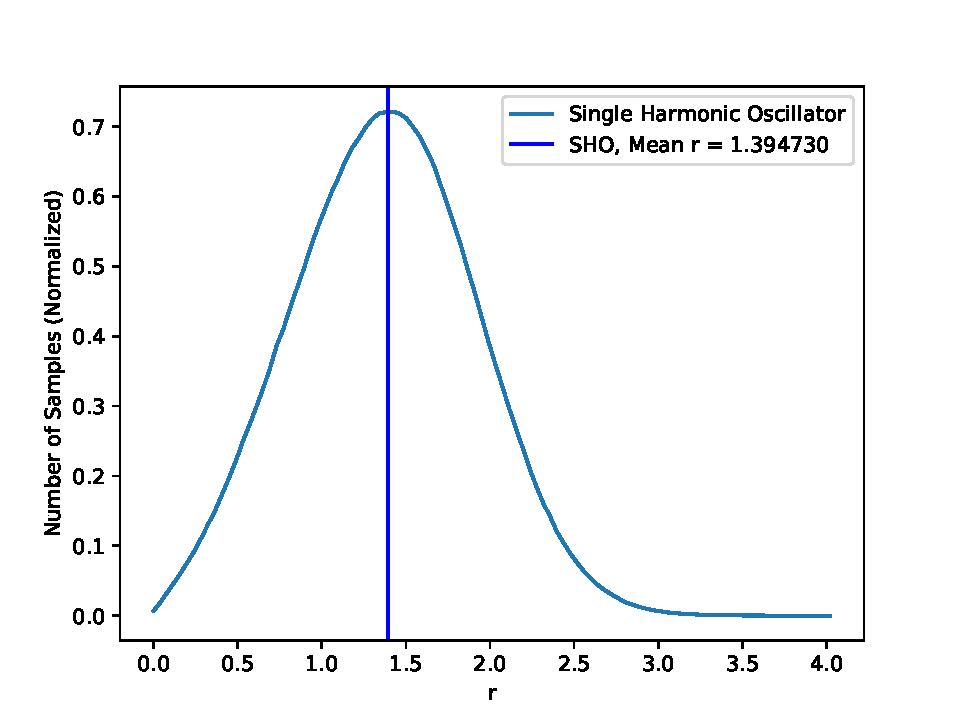
\includegraphics[width=\linewidth]{figures/densitySHO/density_SHO_N6_Omega1_2d}
\caption{$N=6$} \label{fig:SHO_N6_2d_a}
\end{subfigure}\hspace*{\fill}
\begin{subfigure}{0.48\textwidth}
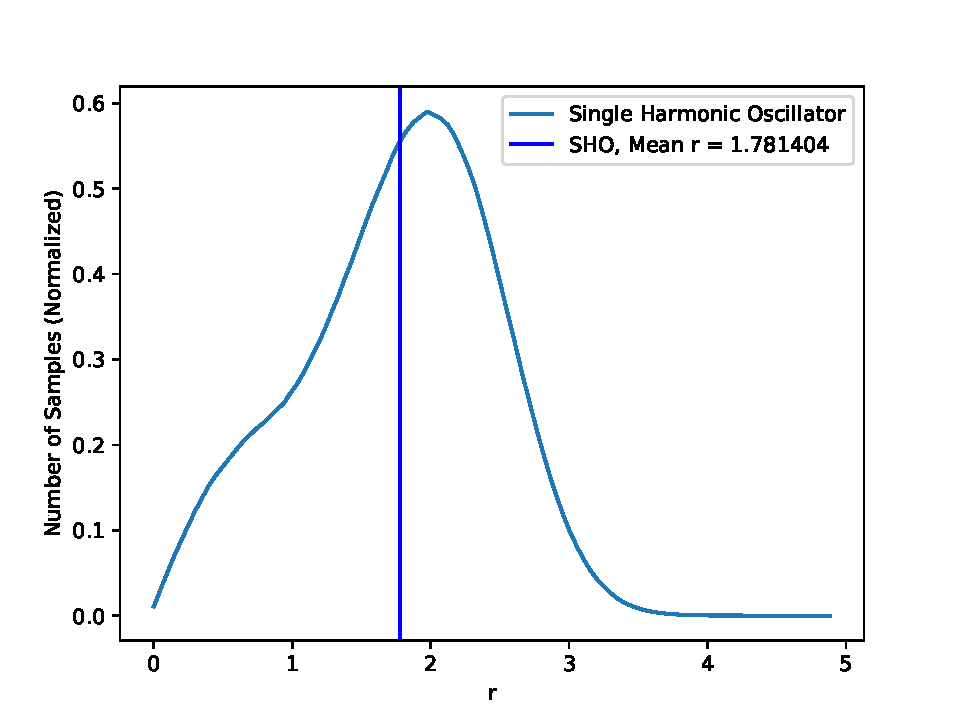
\includegraphics[width=\linewidth]{figures/densitySHO/density_SHO_N12_Omega1_2d}
\caption{$N=12$} \label{fig:SHO_N12_2d_b}
\end{subfigure}

\medskip
\begin{subfigure}{0.48\textwidth}
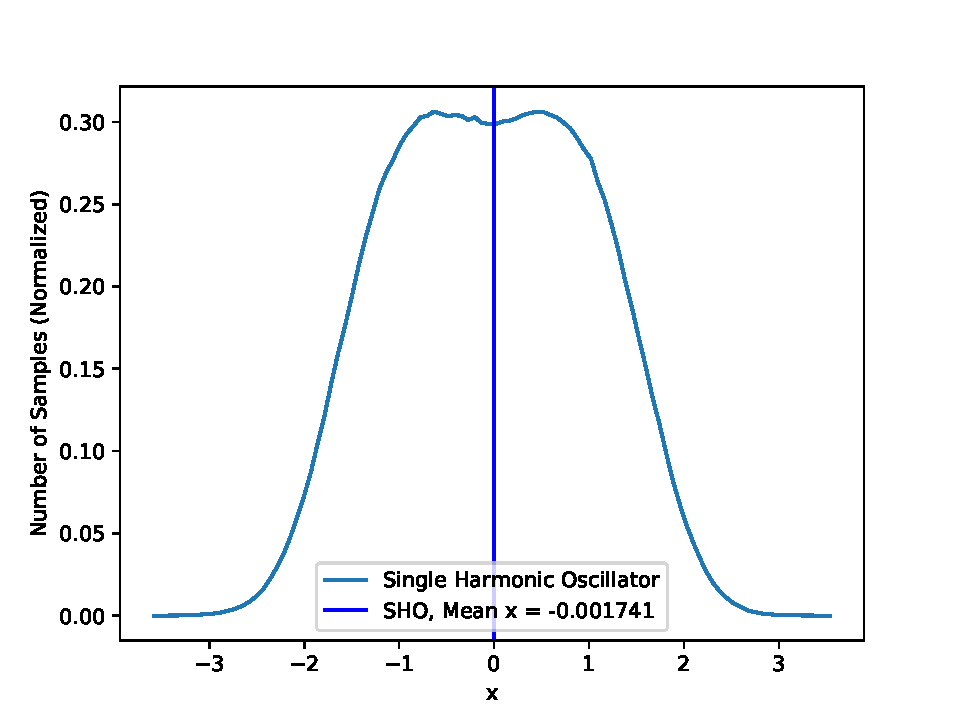
\includegraphics[width=\linewidth]{figures/densitySHO/density_SHO_N6_Omega1_2d_x}
\caption{$N=6$} \label{fig:SHO_N6_2d_x_c}
\end{subfigure}\hspace*{\fill}
\begin{subfigure}{0.48\textwidth}
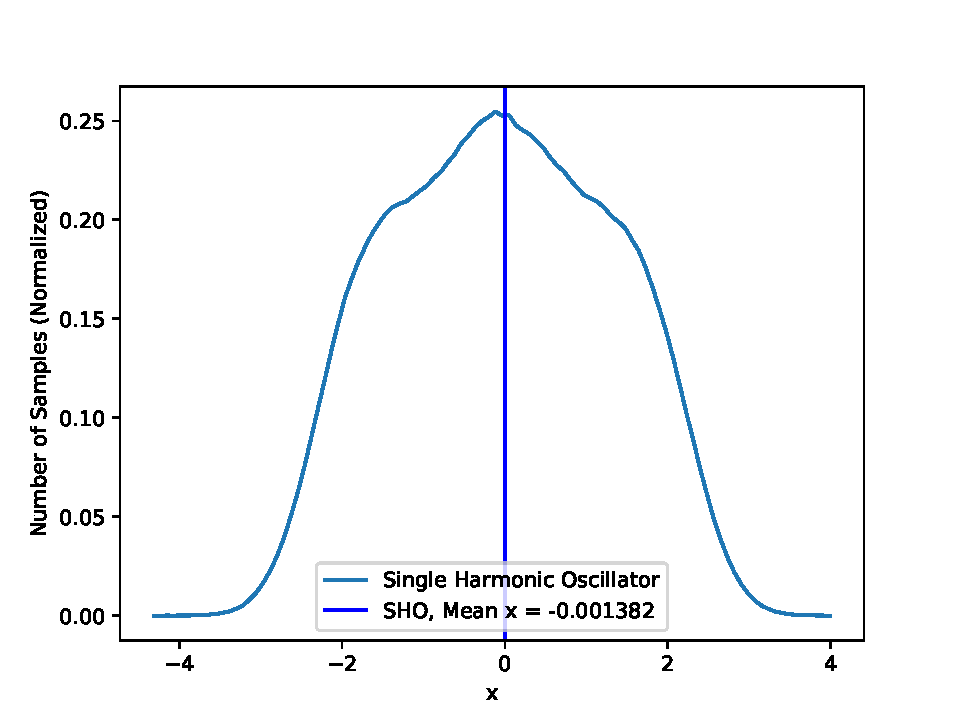
\includegraphics[width=\linewidth]{figures/densitySHO/density_SHO_N12_Omega1_2d_x}
\caption{$N=12$} \label{fig:SHO_N12_2d_x_d}
\end{subfigure}

\medskip
\begin{subfigure}{0.48\textwidth}
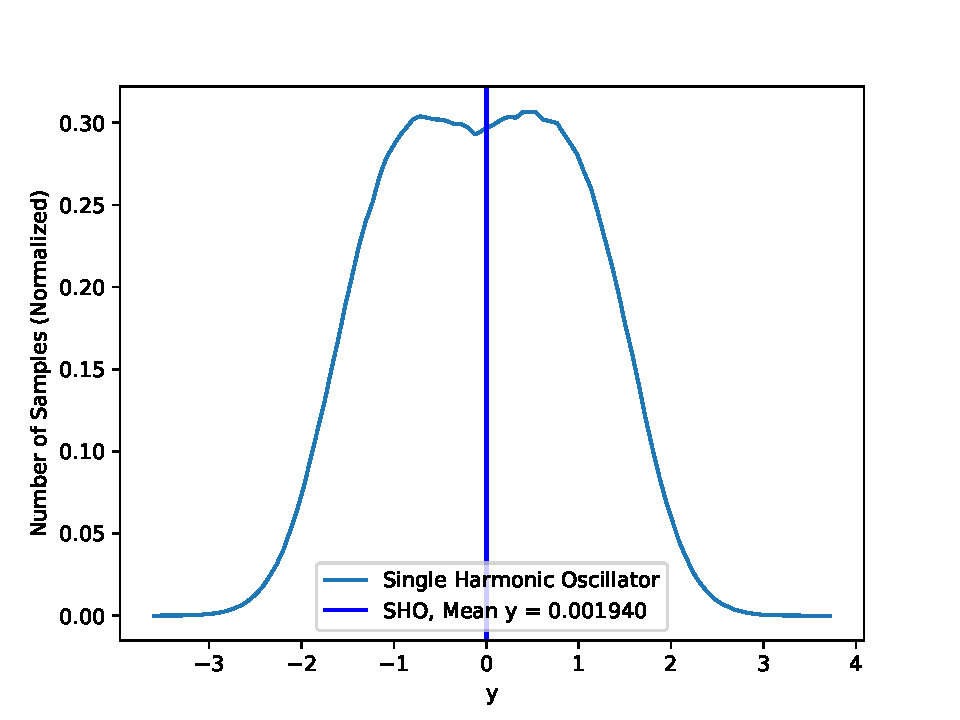
\includegraphics[width=\linewidth]{figures/densitySHO/density_SHO_N6_Omega1_2d_y}
\caption{$N=6$} \label{fig:SHO_N6_2d_y_e}
\end{subfigure}\hspace*{\fill}
\begin{subfigure}{0.48\textwidth}
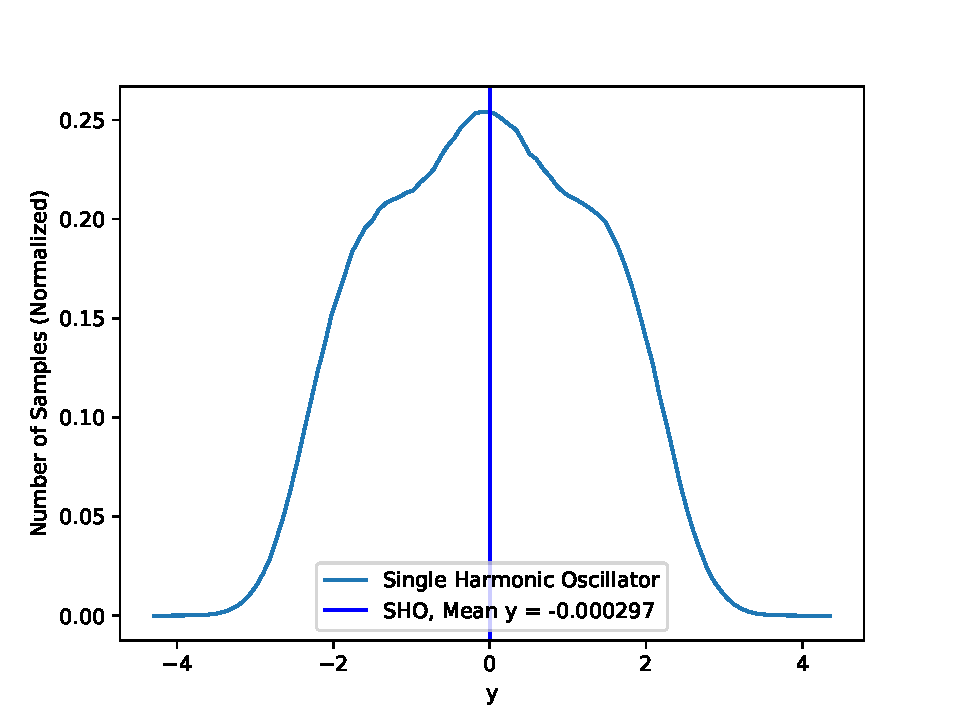
\includegraphics[width=\linewidth]{figures/densitySHO/density_SHO_N12_Omega1_2d_y}
\caption{$N=12$} \label{fig:SHO_N12_2d_y_f}
\end{subfigure}

\caption{Figures \ref{fig:SHO_N6_2d_a} and \ref{fig:SHO_N12_2d_b} show the one-body densities of a two-dimensional single harmonic oscillator with $N$ particles and $\omega=1$. The other figures show the corresponding distributions of $x$ and $y$ positions individually. The $x$ and $y$ distributions are almost identical due to the harmonic oscillator potential being symmetric.} \label{fig:SHO_density2d}
\end{figure}


\begin{figure}
\centering
\begin{subfigure}{0.48\textwidth}
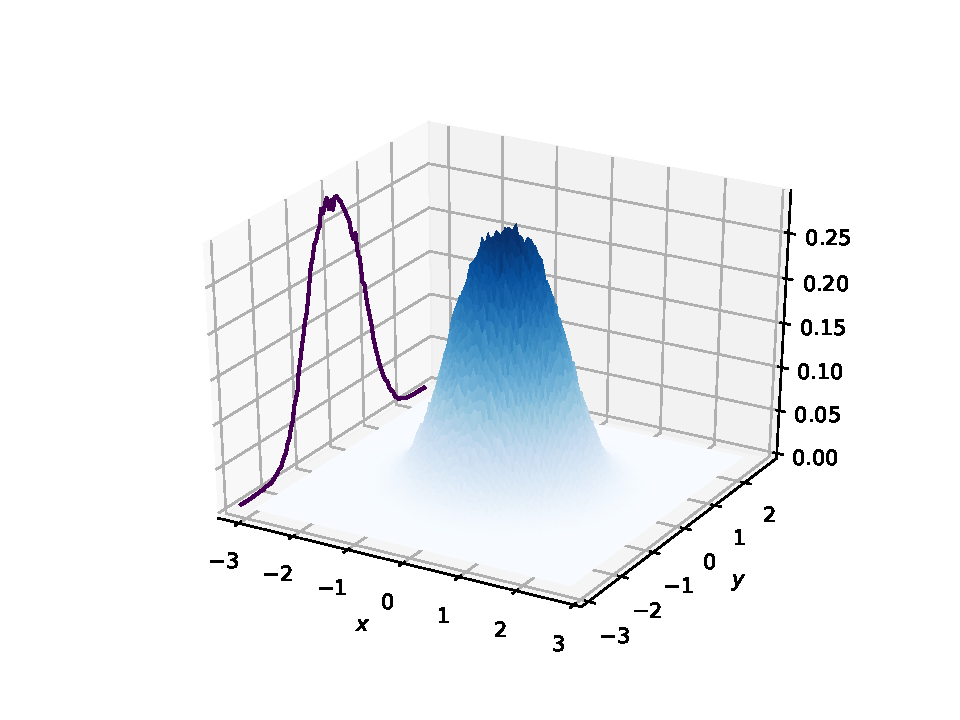
\includegraphics[width=\linewidth]{figures/densitySHO/density3D_SHO_N2_Omega1_2d}
\caption{$N=2$} \label{fig:SHO_density3D_N2_a}
\end{subfigure}\hspace*{\fill}
\begin{subfigure}{0.48\textwidth}
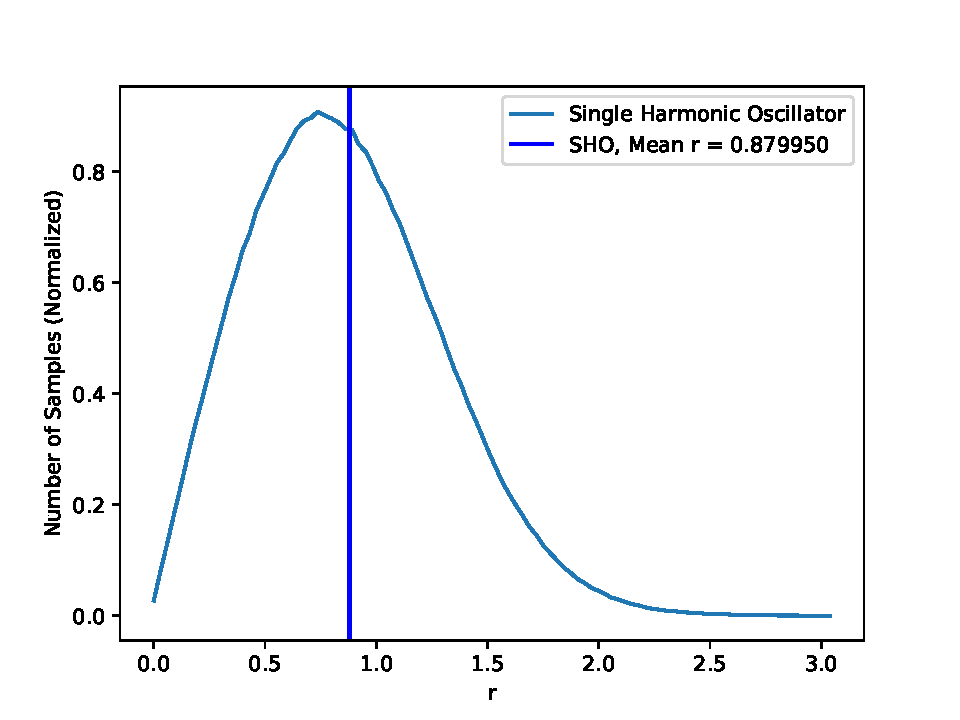
\includegraphics[width=\linewidth]{figures/densitySHO/density_SHO_N2_Omega1_2d}
\caption{$N=2$} \label{fig:SHO_density_N2_b}
\end{subfigure}

\medskip
\begin{subfigure}{0.48\textwidth}
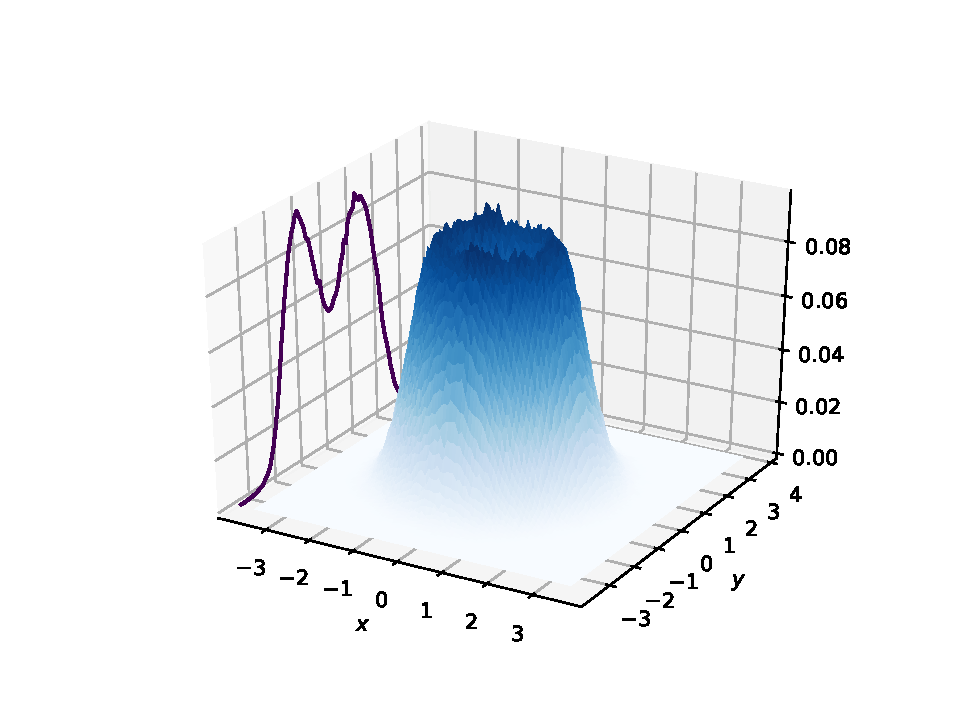
\includegraphics[width=\linewidth]{figures/densitySHO/density3D_SHO_N6_Omega1_2d}
\caption{$N=6$} \label{fig:SHO_density3D_N6_c}
\end{subfigure}\hspace*{\fill}
\begin{subfigure}{0.48\textwidth}
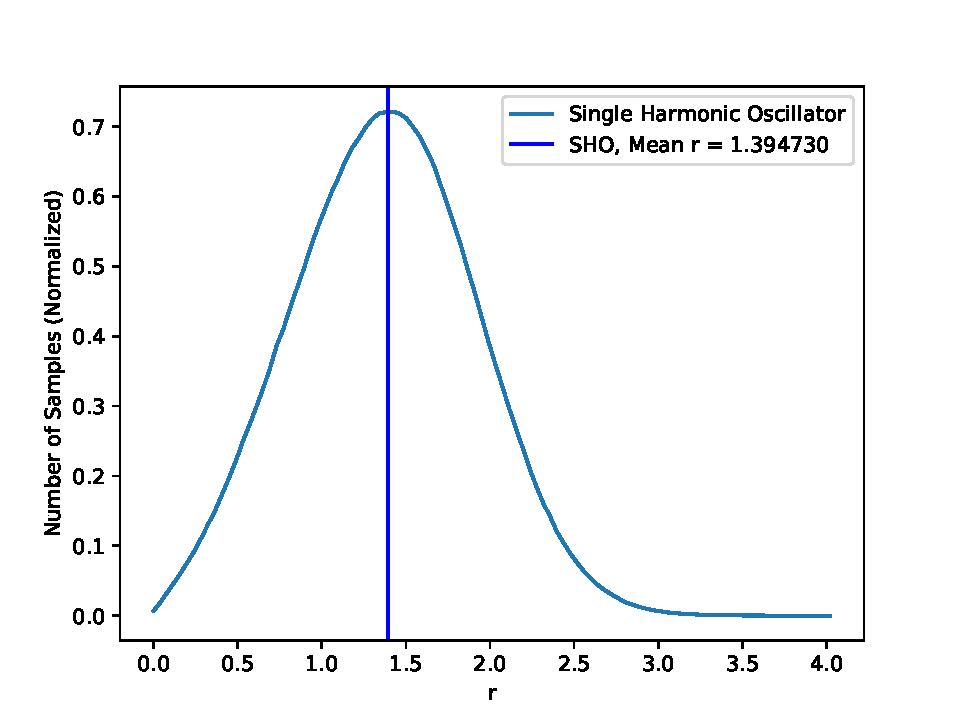
\includegraphics[width=\linewidth]{figures/densitySHO/density_SHO_N6_Omega1_2d}
\caption{$N=6$} \label{fig:SHO_density_N6_d}
\end{subfigure}

\medskip
\begin{subfigure}{0.48\textwidth}
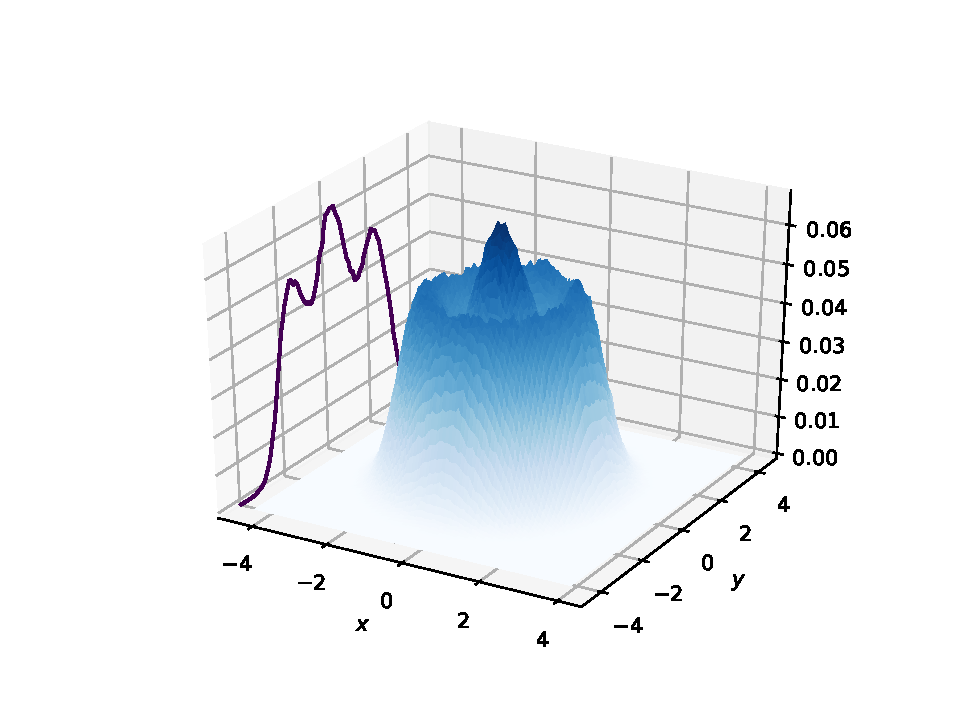
\includegraphics[width=\linewidth]{figures/densitySHO/density3D_SHO_N12_Omega1_2d}
\caption{$N=12$} \label{fig:SHO_density3D_N12_e}
\end{subfigure}\hspace*{\fill}
\begin{subfigure}{0.48\textwidth}
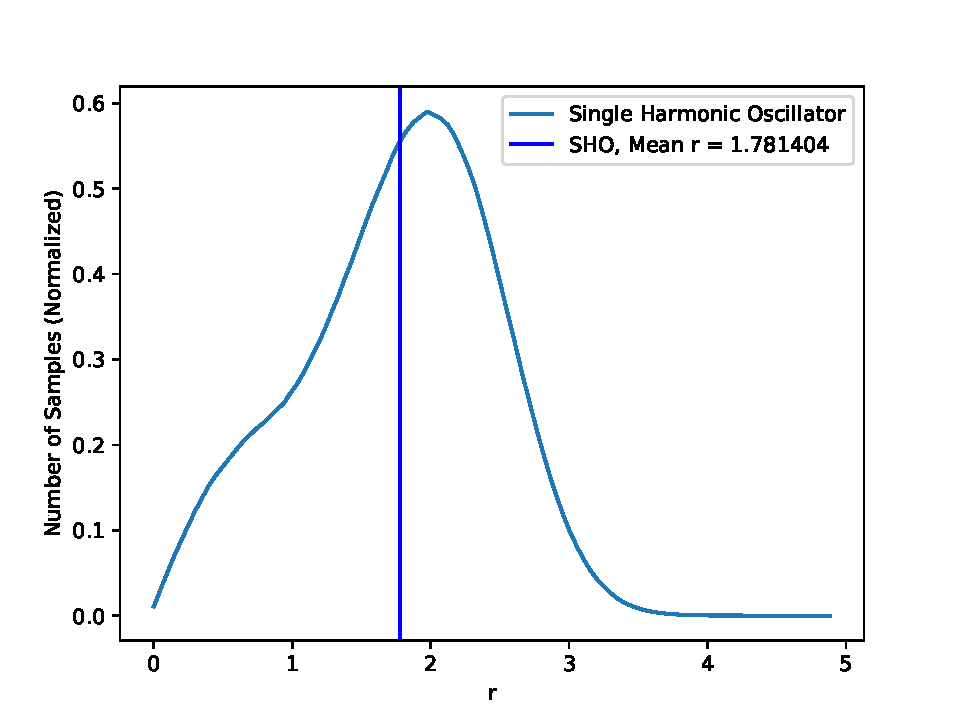
\includegraphics[width=\linewidth]{figures/densitySHO/density_SHO_N12_Omega1_2d}
\caption{$N=12$} \label{fig:SHO_density_N12_f}
\end{subfigure}

\caption{The right-hand side shows the one-body densities of a two-dimensional single harmonic oscillator with $N$ particles and $\omega=1$. The left-hand side shows the distribution of positions for a mesh-grid of the $x$ and $y$ positions. From the left-hand side we can clearly see that the particles are divided into more energy levels as $N$ increases.} \label{fig:SHO_density3D_2d}
\end{figure}


\section{Double Harmonic Oscillator Well}

In this section we look at systems of particles in a double harmonic oscillator potential well, where the distance between the center of each well and the barrier between the wells is $L_x = 1$. We look at energies and one-body densities in both two and three dimensions.

\subsection{Ground State Energies}

Unlike for the single harmonic oscillator well, for the double harmonic oscillator well we have no reason to expect the results we get when the single particle wave functions are approximated by expansion in a single harmonic oscillator basis ($E_\textrm{coeff}$), to be exactly equal to the result from using harmonic oscillator single particle wave functions directly ($E_\textrm{reg}$). This is because the basis functions are still single harmonic oscillator functions, but the single particle wave functions we are trying to approximate are for a double harmonic oscillator well, so they are not of the same type as the basis functions. Because of this we should also expect to need more basis functions to get good results. Of course the $\alpha$ dependence discussed in Section \ref{sec: SHO GSE} is still missing from the coefficients. We compare $E_\textrm{coeff}$ with $E_\textrm{reg}$, and see that they are reasonably consistent with each other provided we use enough basis functions when calculating $E_\textrm{coeff}$.

\subsubsection{Two Dimensions}

The ground state energies of systems with various numbers of particles $N$ and harmonic oscillator frequencies $\omega$ are listed in Table \ref{tab: EnergiesDHO2D}. In most cases we need more basis functions to get good results for the double harmonic oscillator well, than we did for the single well, which is to be expected since the basis functions are single well functions. From the table we see that with a reasonable amount of basis functions we can achieve consistency between $E_\textrm{coeff}$ and $E_\textrm{reg}$. Unlike for the single well, here we only have one benchmark to compare our results to. In order to compare with the benchmark we have used the same distance between the wells as was used for the benchmark, i.e. $R=2$ in the $x$-direction, which corresponds to $L_x = 1$ in our case. From the table we see that our results are fairly consistent with the benchmark, but just as for the single well case, there are some difference likely due to some difference in the variational parameters.

For $N=2$ and $N=12$ we can directly compare the results of Table \ref{tab: EnergiesDHO2D} with those from Table \ref{tab: EnergiesSHO2D}. We see that given the same number of particles and the same $\omega$ the double well results are always smaller than their single well counterparts. This is expected since the particles are split between two wells in the double well. For example let us look at the $N=2$, $\omega = 1$ case. If $L_x$ was equal to $0$ the wells would be on top of each other, which means we essentially would have a single well potential, and the energy for a interacting system would then be $E=3$. If on the other hand $L_x$ was approaching infinity, then (assuming one particle in each well) the system could be considered as two independent single wells with one particle and consequently no interaction, and the energy would then be $E=2$. So for our case with $L_x=1$ we should expect $2<E<3$, and indeed we get $E_\textrm{coeff}=2.326$. If we imagine the $12$ particle case with $L_x$ approaching infinity there would still be interaction in each well, since there would be $6$ particles in each. However, for $N=6$, $\omega=1$ in Table \ref{tab: EnergiesSHO2D}, we have that $E_\textrm{coeff}=20.243$, so for the double well with $12$ particles and $L_x \rightarrow \infty$ the energy would be $E \approx 2\times 20.243 = 40.486$. Again the $L_x=0$ case corresponds to a single well with $12$ particles and for that we have the result $E_\textrm{coeff}=65.952$ from Table \ref{tab: EnergiesSHO2D}. So for the double well with $N=12$, $\omega=1$ we should expect $40.486<E<65.952$, and indeed we get $E_\textrm{coeff}=55.165$.

One thing to note about this is that while the double well results are smaller than the single well results in all cases, the difference between the two becomes very small as $\omega$ decreases. If we look at the $N=2$, $\omega=0.01$ case we see that for the single well we have $E_\textrm{coeff}=0.0754$ while for the double well we have $E_\textrm{coeff}=0.0735$. The reason for this is that as $\omega$ decreases the barrier between the wells in the double well becomes smaller and smaller, due to the widening of the wells. When this happens the double well starts to look more and more like a single well (though with an extended bottom). This is shown in Figure \ref{fig:DW}.

\begin{table}[!ht]
  \centering
  \begin{tabular}{c c c c c c}
    \hline
    \hline
    $N$ & $\omega$ & Basis Functions & $E_\textrm{coeff}$ & $E_\textrm{reg}$ & $E_\textrm{ref}$ \\*
    \hline
    2 & 0.01 & 1 & 0.0735(3) & 0.0727(2) & - \\*
      & 0.10 & 1 & 0.4106(9) & 0.4018(7) & -  \\*
      & 0.28 & 6 & 0.860(1) & 0.866(2) & - \\*
      & 0.50 & 6 & 1.336(2) & 1.339(2) & - \\*
      & 1.00 & 15 & 2.326(2) & 2.321(2) & 2.3496(1) \vspace{2 mm}\\*
      
    4 & 0.10 & 3 & 1.5966(9) & 1.5886(7) & - \\*
      & 0.28 & 10 & 3.362(1) & 3.222(1) & - \\*
      & 0.50 & 55 & 4.958(2) & 4.831(2) & - \\*
      & 1.00 & 55 & 7.850(2) & 7.848(2) & - \vspace{2 mm}\\*
      
    12 & 0.10 & 21 & 12.106(6) & 12.034(6) & - \\*
       & 0.28 & 21 & 23.771(6) & 23.785(7) & - \\*
       & 0.50 & 36 & 34.945(5) & 34.945(6) & - \\*
       & 1.00 & 45 & 55.165(6) & 55.226(6) & - \\*
    \hline
    \hline
  \end{tabular}
  \caption{The table lists ground state energy results for various double harmonic oscillator systems in two dimensions, and corresponding benchmarks. $N$ is the number of particles and $\omega$ is the harmonic oscillator frequency. $E_\textrm{coeff}$ are the energies obtained when the single particle wave functions are approximated by expansion in a single harmonic oscillator basis. $E_\textrm{reg}$ are the energies obtained when using double harmonic oscillator single particle wave functions directly. The benchmark is from J. Høgberget \cite{Jorgen} (DMC). The numbers in parenthesis are the statistical errors found using blocking.}
  \label{tab: EnergiesDHO2D}
\end{table}

\begin{figure}[!ht]
\centering
\begin{subfigure}{0.48\textwidth}
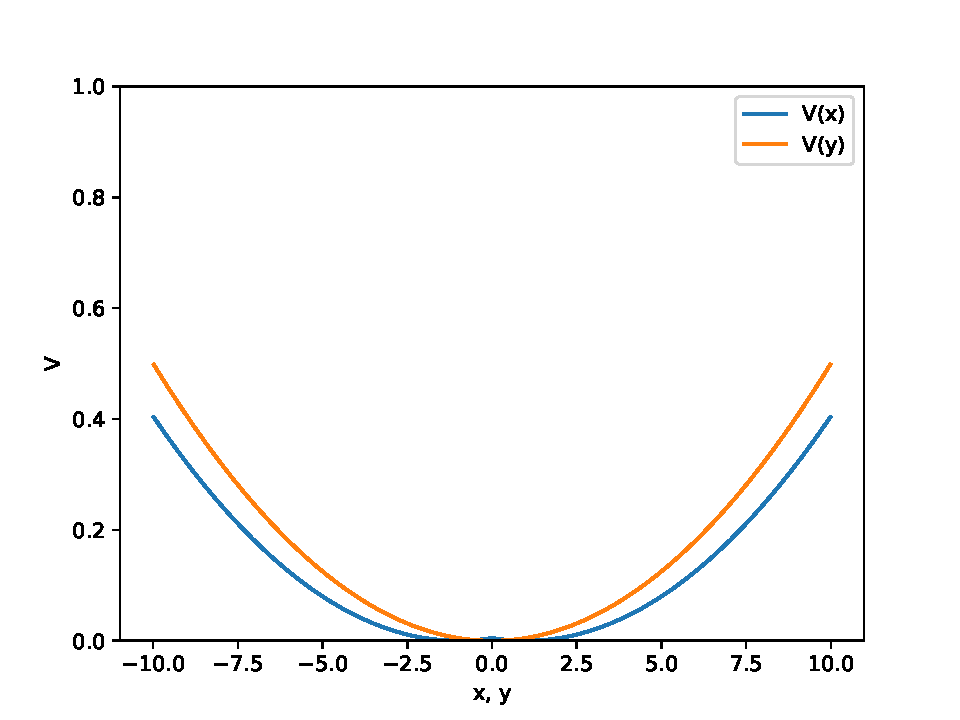
\includegraphics[width=\linewidth]{figures/DW_omega01}
\caption{$\omega=0.1$} \label{fig:DW_01}
\end{subfigure}\hspace*{\fill}
\begin{subfigure}{0.48\textwidth}
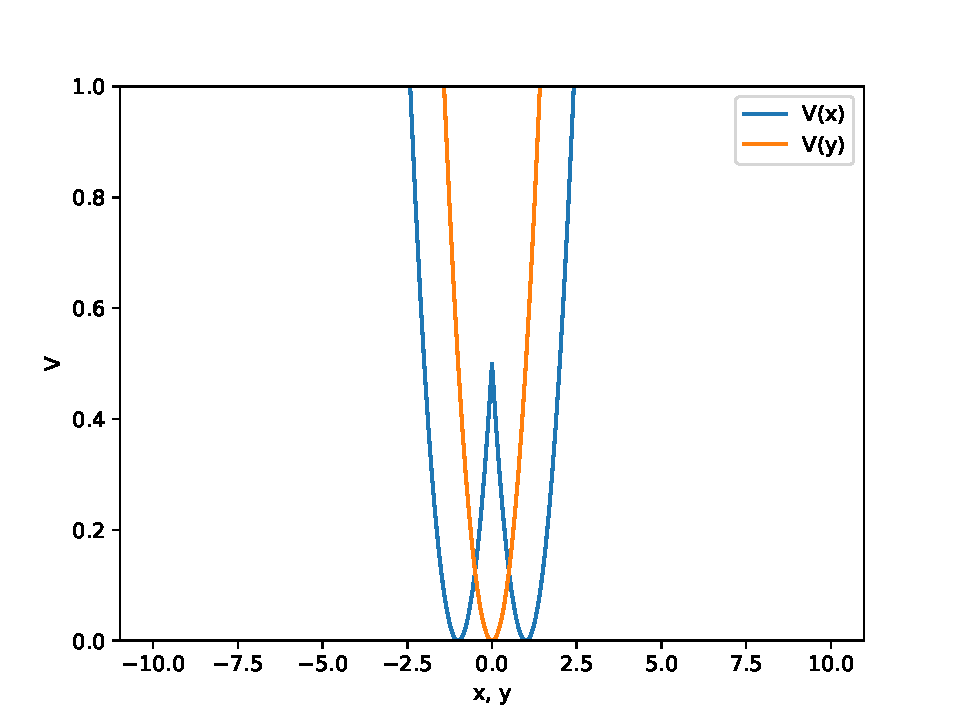
\includegraphics[width=\linewidth]{figures/DW_omega1}
\caption{$\omega=1$} \label{fig:DW_1}
\end{subfigure}

\caption{The shape of a double well potential with centers at $x=\pm1$ and $y=0$, for $\omega=0.1$ and $\omega=1$ with constant axes so they can be compared. $V(x)$ is the potential in the $x$-direction (double well) and $V(y)$ in the $y$-direction (single well). We see that for lower $\omega$, $V(x)$ is more similar to $V(y)$, indicating that the double well potential becomes more similar to a single well potential as $\omega$ decreases.} \label{fig:DW}
\end{figure}

\subsubsection{Three Dimensions}

The ground state energies for the three-dimensional case are listed in Table \ref{tab: EnergiesDHO3D}. For the three-dimensional case we do not have any benchmarks to compare our results with. However, we can still compare the results with each other, and from the table we see that $E_\textrm{coeff}$ and $E_\textrm{reg}$ are reasonably consistent with each other. In general we need more basis function to achieve good results for $E_\textrm{coeff}$, than we did in two dimensions. We also see that the similarities between the single well and the double well we observed in the two-dimensional case when $\omega$ was small, is also present in the three-dimensional case. As expected the energy is also generally larger for the three-dimensional case than for the two-dimensional case.

\begin{table}[!ht]
  \centering
  \begin{tabular}{c c c c c}
    \hline
    \hline
    $N$ & $\omega$ & Basis Functions & $E_\textrm{coeff}$ & $E_\textrm{reg}$ \\*
    \hline
    2 & 0.01 & 1 & 0.0782(2) & 0.0779(2) \\*
      & 0.10 & 10 & 0.4639(4) & 0.4652(5) \\*
      & 0.28 & 10 & 1.0642(7) & 1.0711(9) \\*
      & 0.50 & 10 & 1.7324(8) & 1.738(1) \\*
      & 1.00 & 35 & 3.212(2) & 3.194(2) \vspace{2 mm}\\*
      
    4 & 0.10 & 10 & 1.640(1) & 1.642(1) \\*
      & 0.28 & 56 & 3.518(1) & 3.483(2) \\*
      & 0.50 & 56 & 5.3858(9) & 5.360(2) \\*
      & 1.00 & 56 & 9.153(2) & 9.106(2) \\*
    \hline
    \hline
  \end{tabular}
  \caption{The table lists ground state energy results for various double harmonic oscillator systems in three dimensions. $N$ is the number of particles and $\omega$ is the harmonic oscillator frequency. $E_\textrm{coeff}$ are the energies obtained when the single particle wave functions are approximated by expansion in a single harmonic oscillator basis. $E_\textrm{reg}$ are the energies obtained when using double harmonic oscillator single particle wave functions directly. The numbers in parenthesis are the statistical errors found using blocking.}
  \label{tab: EnergiesDHO3D}
\end{table}


\subsection{One-Body Densities}

We are interested in looking at how particles are distributed in a double harmonic oscillator well. Just as for the single well, the particles will push each other away from the center, but here we do not just have a center for each well, we have a center between them at the potential barrier. We have placed this center at $r=0$, and each well center is a distance $r=1$ away. Going forward we will refer to this center as the system center. If there was no interaction between particles we would expect the particles to gather at the bottom of each well where the external potential is smallest. Since we have a repulsive interaction between the particles we expect the particles to push each other away from the well centers, just as we saw for the single well. Unlike for the single well, the well centers and the system center do not overlap for the double well so the mean distance between particles and the system center should be greater than an equivalent single well system. By comparing Figure \ref{fig:DHO_N12_2d_b} and \ref{fig:SHO_N12_2d_b} we see that for $N=12$ the mean value of $r$ is greater for a double well than for a single well. Just as for the single well, we also see that when going from $4$ particles to $12$ particles the mean value of $r$ increases.

In addition if we look at all particles in one well as a group, then that group should push the particles in the other well away from the system center and vice versa. This can be seen clearly from Figure \ref{fig:DHO_density3D_a} and \ref{fig:DHO_density3D_b}. In Figure \ref{fig:DHO_density3D_a} we have $N=2$ and one particle in each well and in Figure \ref{fig:DHO_density3D_b} we have $N=4$ and two particles in each well. In both cases the distribution ends up with one top for each well, however for the $N=4$ case the gap between the tops is larger and the distribution at the system center is smaller (as seen from the graph behind the surface plot). This is because when $N=4$ we have two groups of two particles pushing each other away from the system center, while in the $N=2$ case each group only has one particle and consequently the force on one group from the other is smaller than in the $N=4$ case.

When we increase the number of particles to $12$ we see from Figure \ref{fig:DHO_density3D_c} and \ref{fig:DHO_density3D_d} that the distribution gets a more interesting shape. For a well with $6$ particles in the single well case we saw from Figure \ref{fig:SHO_density3D_N6_c} that the distribution got a volcano like shape. However, when we have a double well with $6$ particles in each well we see from Figure \ref{fig:DHO_density3D_d} that the interaction force from one well on the other causes the volcano like shape to change into three tops surrounding the well center. The three tops are positioned as far away from each other as they can, and between the tops the distribution is somewhat smaller, but still fairly large.

In Figure \ref{fig:DHO_density2d} we have plots of the $x$ distribution and $y$ distribution separately for $N=4$ and $N=12$. The single well was symmetric so the distributions were identical in that case, but for the double well, we have a double well potential in the $x$-direction and a single well potential in the $y$-direction. The $y$ distributions get the same shape as they did for half as many particles in a single well (since each well has $N/2$ particles). The $x$ distributions however, get new shapes which clearly show that we have two identical wells separated by a barrier at $x=0$.

\begin{figure}[!ht]
\centering
\begin{subfigure}{0.48\textwidth}
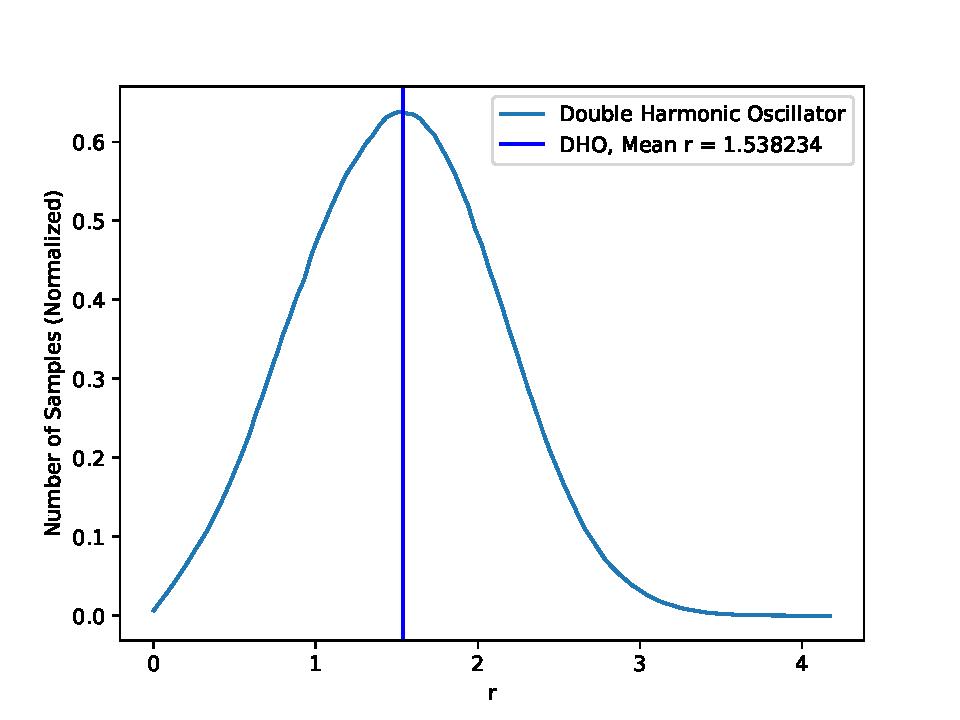
\includegraphics[width=\linewidth]{figures/densityDHO/density_DHO_N4_Omega1_2d}
\caption{$N=4$} \label{fig:DHO_N4_2d_a}
\end{subfigure}\hspace*{\fill}
\begin{subfigure}{0.48\textwidth}
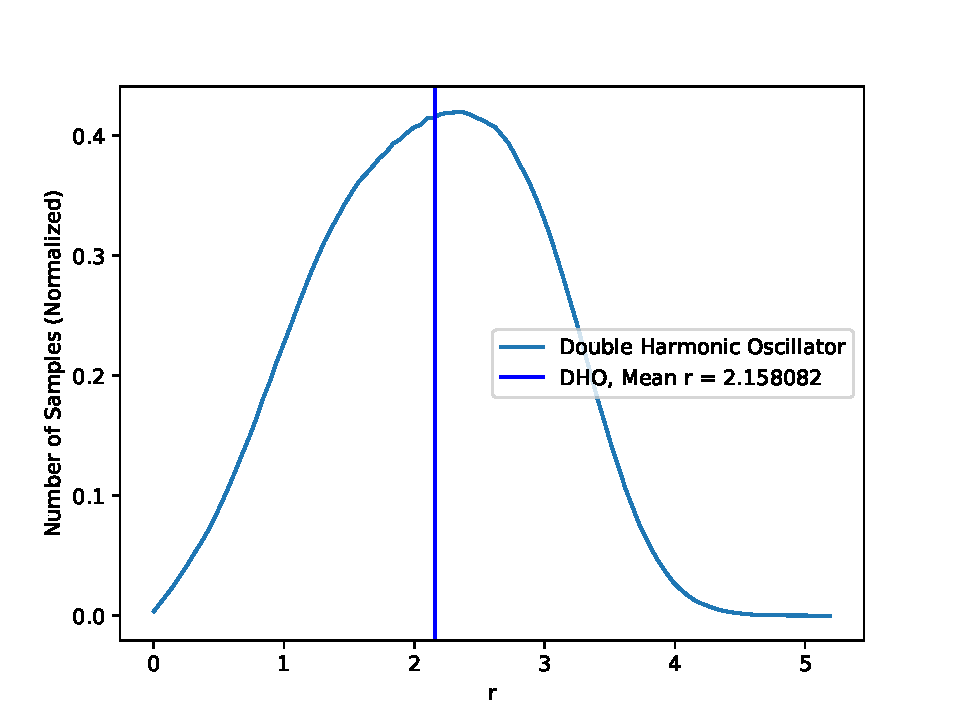
\includegraphics[width=\linewidth]{figures/densityDHO/density_DHO_N12_Omega1_2d}
\caption{$N=12$} \label{fig:DHO_N12_2d_b}
\end{subfigure}

\medskip
\begin{subfigure}{0.48\textwidth}
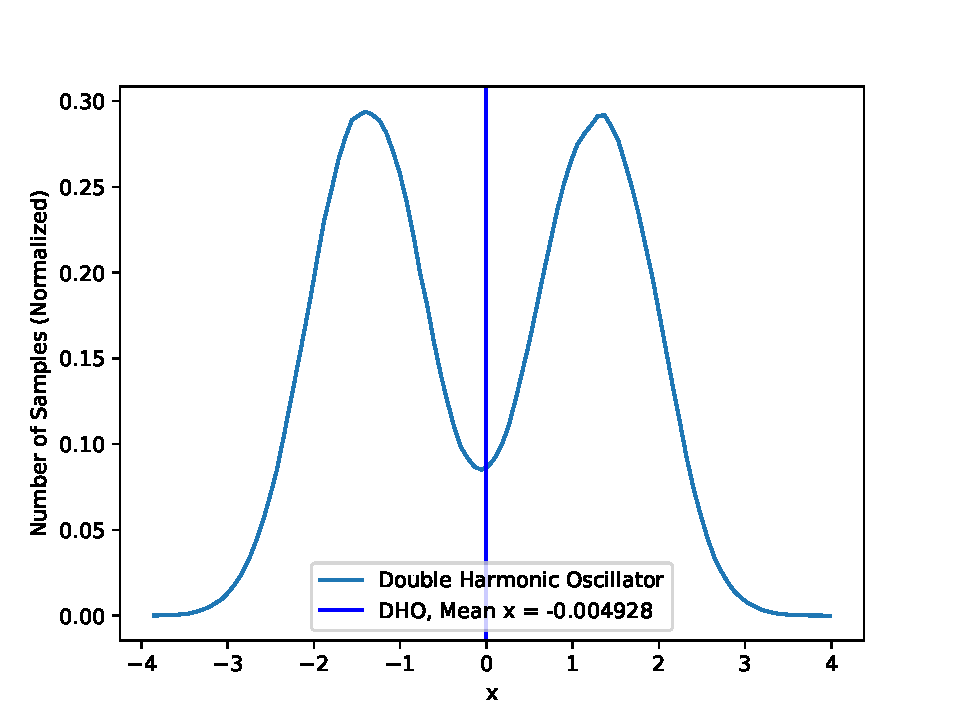
\includegraphics[width=\linewidth]{figures/densityDHO/density_DHO_N4_Omega1_2d_x}
\caption{$N=4$} \label{fig:DHO_N4_2d_x_c}
\end{subfigure}\hspace*{\fill}
\begin{subfigure}{0.48\textwidth}
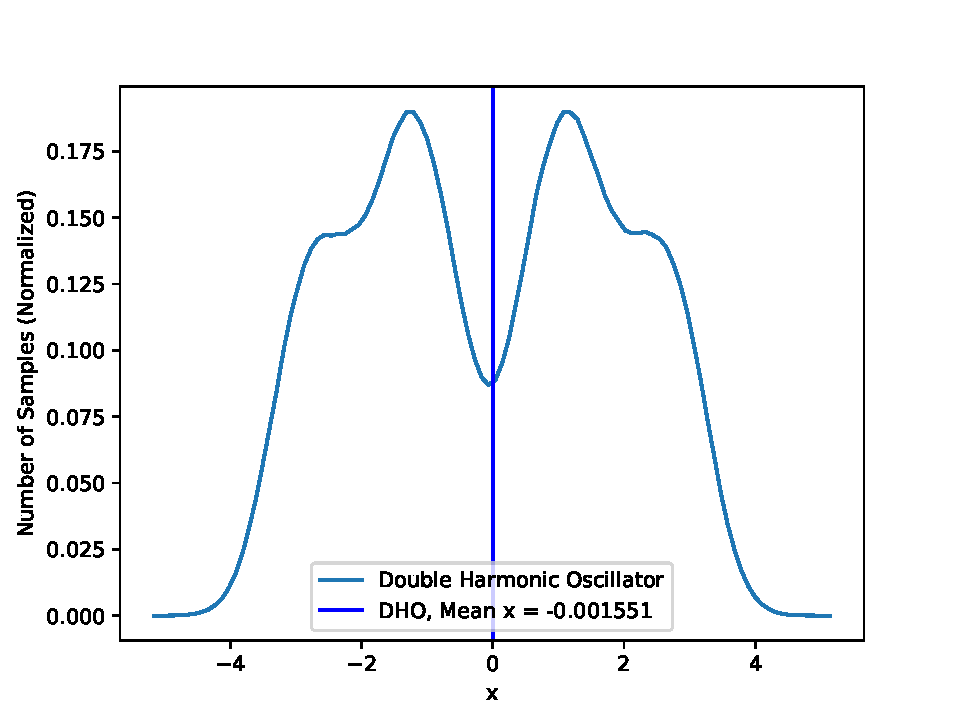
\includegraphics[width=\linewidth]{figures/densityDHO/density_DHO_N12_Omega1_2d_x}
\caption{$N=12$} \label{fig:DHO_N12_2d_x_d}
\end{subfigure}

\medskip
\begin{subfigure}{0.48\textwidth}
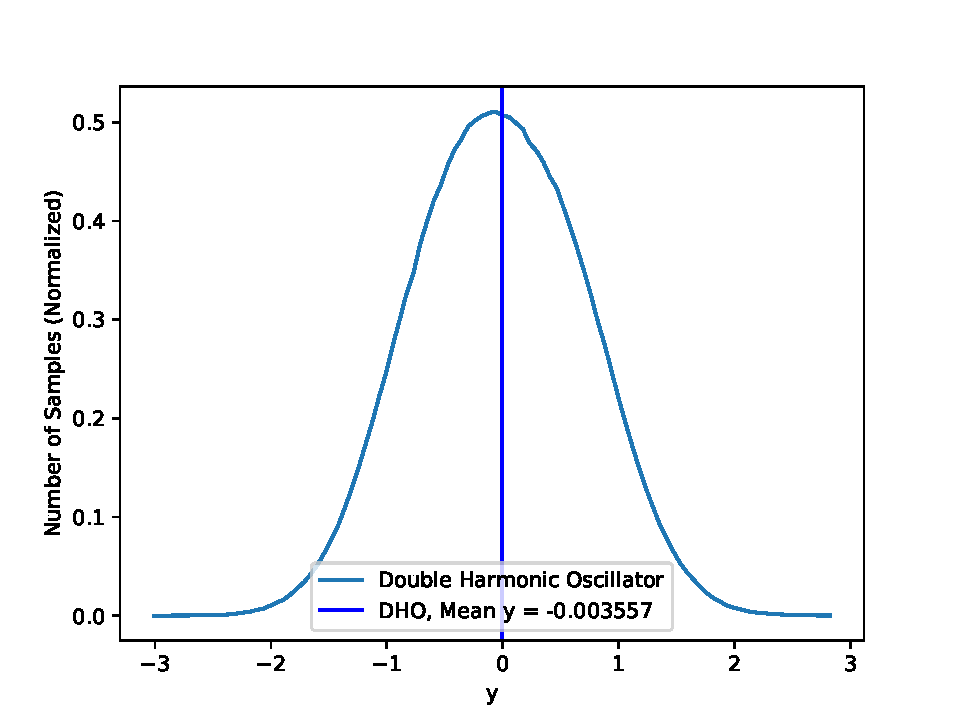
\includegraphics[width=\linewidth]{figures/densityDHO/density_DHO_N4_Omega1_2d_y}
\caption{$N=4$} \label{fig:DHO_N4_2d_y_e}
\end{subfigure}\hspace*{\fill}
\begin{subfigure}{0.48\textwidth}
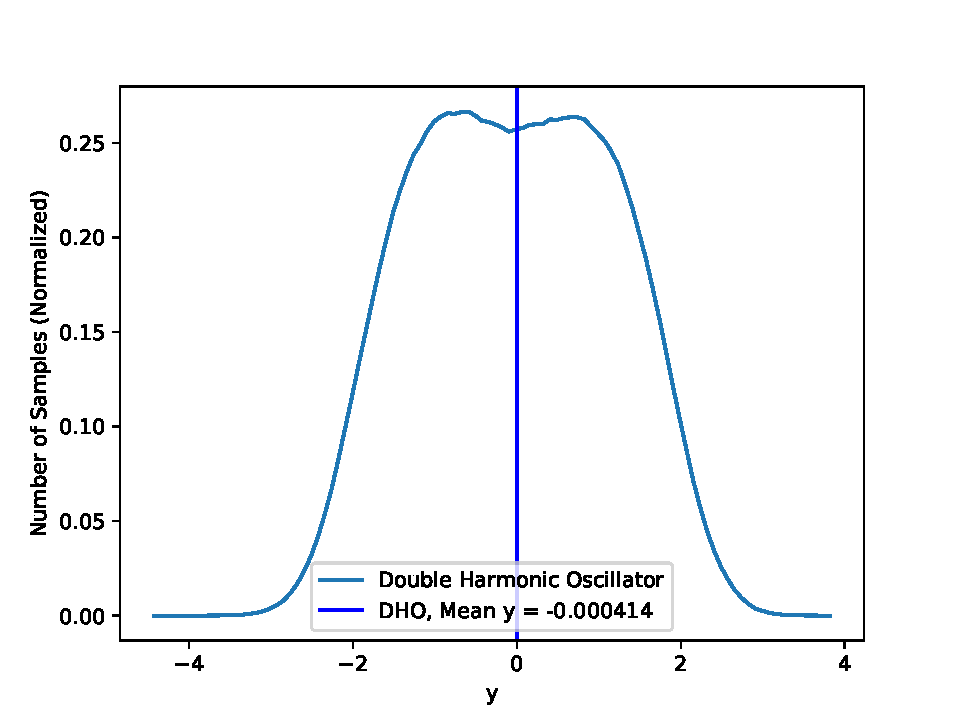
\includegraphics[width=\linewidth]{figures/densityDHO/density_DHO_N12_Omega1_2d_y}
\caption{$N=12$} \label{fig:DHO_N12_2d_y_f}
\end{subfigure}

\caption{Figure \ref{fig:DHO_N4_2d_a} and \ref{fig:DHO_N12_2d_b} show the one-body densities of a two-dimensional double harmonic oscillator with with centers at $x=\pm1$ and $y=0$, $N$ particles and $\omega=1$. The other figures show the corresponding distributions of $x$ and $y$ positions individually. Unlike the single well, the double well is not symmetric, so the $x$ and $y$ distributions are not identical.} \label{fig:DHO_density2d}
\end{figure}



\begin{figure}[!ht]
\centering
\begin{subfigure}{0.48\textwidth}
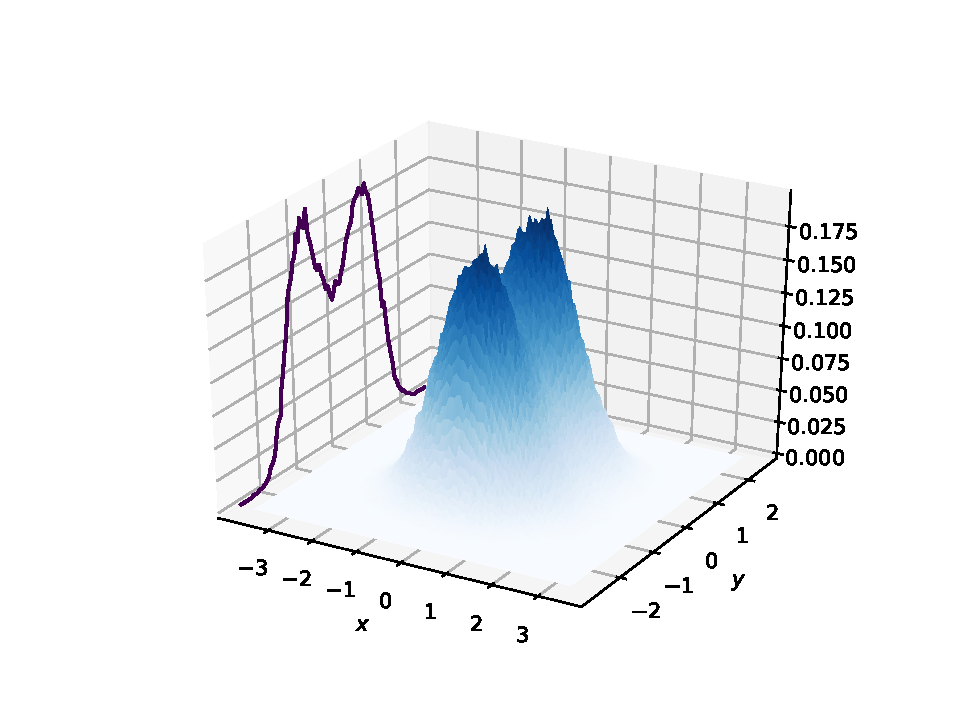
\includegraphics[width=\linewidth]{figures/densityDHO/density3D_DHO_N2_Omega1_2d}
\caption{$N=2$} \label{fig:DHO_density3D_a}
\end{subfigure}\hspace*{\fill}
\begin{subfigure}{0.48\textwidth}
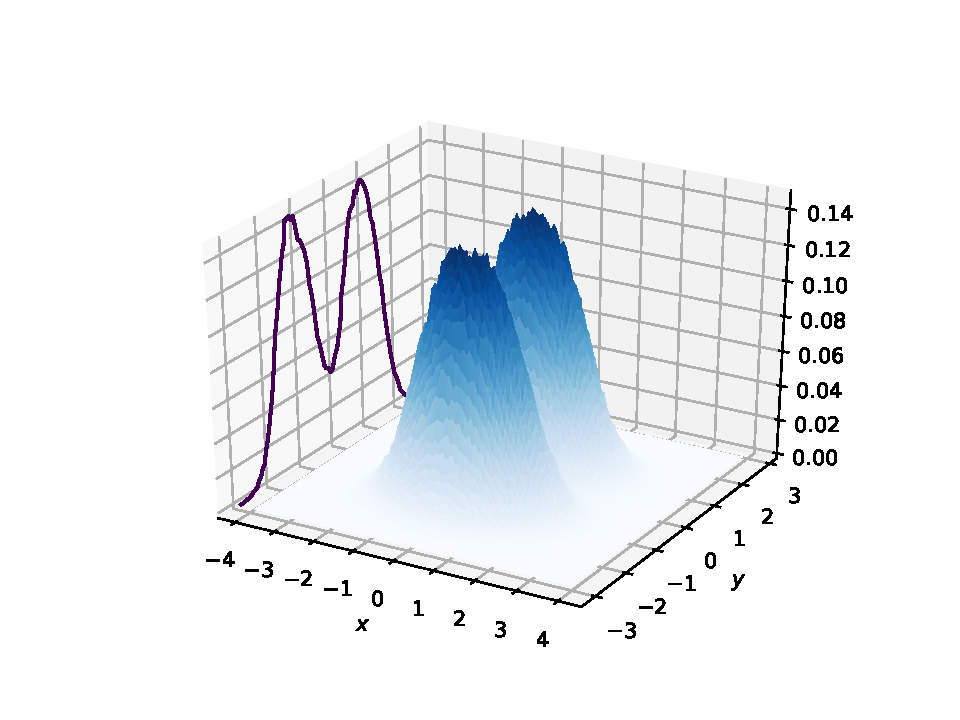
\includegraphics[width=\linewidth]{figures/densityDHO/density3D_DHO_N4_Omega1_2d}
\caption{$N=4$} \label{fig:DHO_density3D_b}
\end{subfigure}

\medskip
\begin{subfigure}{0.48\textwidth}
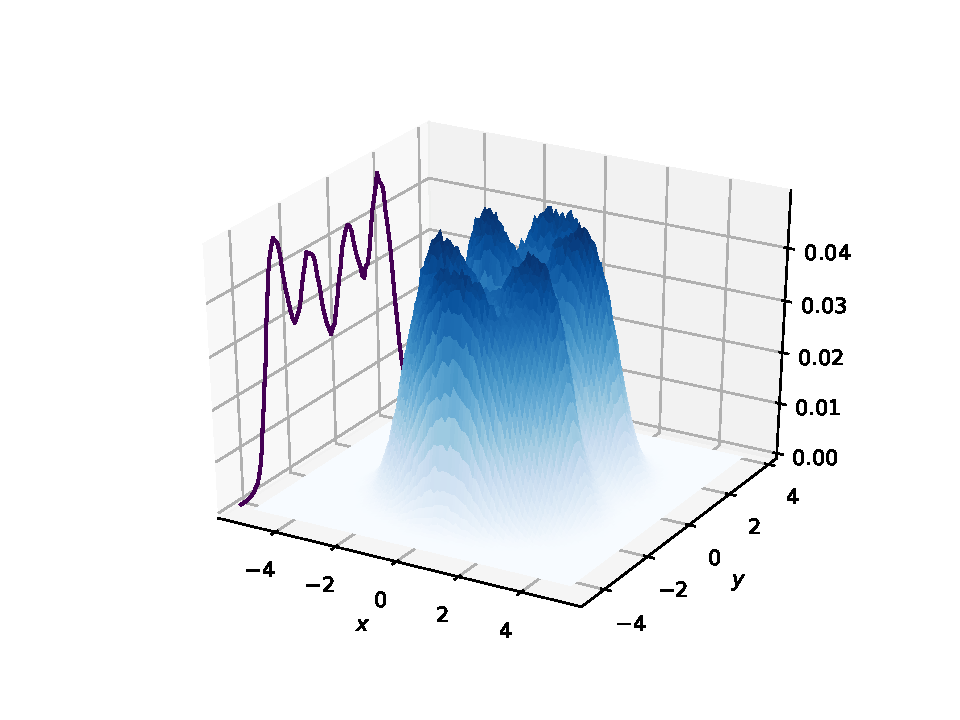
\includegraphics[width=\linewidth]{figures/densityDHO/density3D_DHO_N12_Omega1_2d}
\caption{$N=12$} \label{fig:DHO_density3D_c}
\end{subfigure}\hspace*{\fill}
\begin{subfigure}{0.48\textwidth}
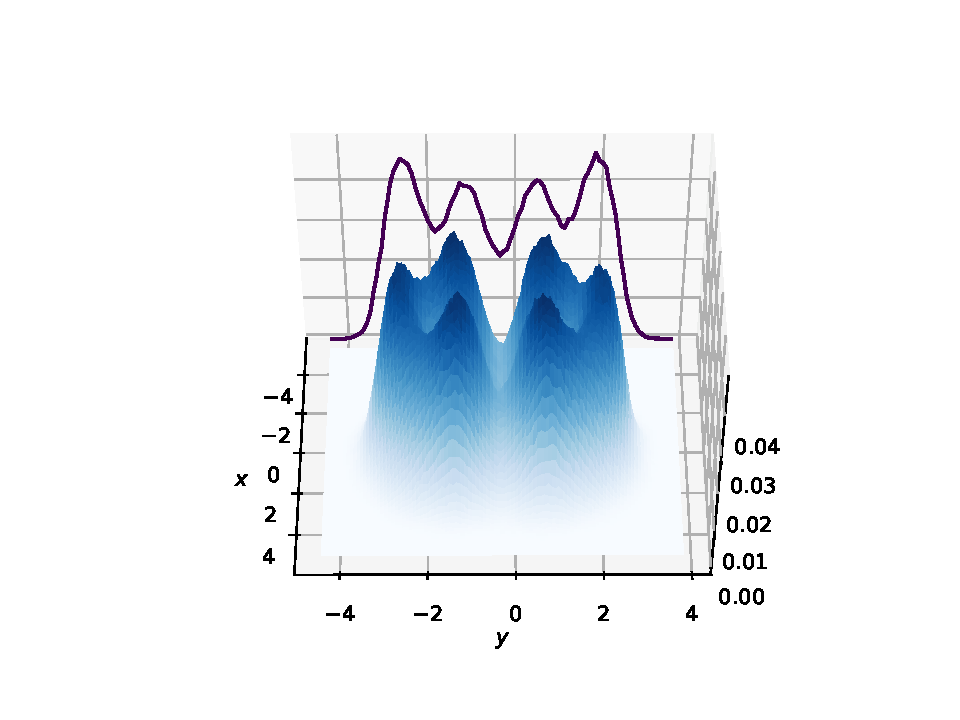
\includegraphics[width=\linewidth]{figures/densityDHO/density3D_DHO_N12_Omega1_2d_v2}
\caption{$N=12$} \label{fig:DHO_density3D_d}
\end{subfigure}

\caption{The figures show the distributions of positions for a mesh-grid of the $x$ and $y$ positions for a double harmonic oscillator well with centers at $x=\pm1$ and $y=0$. The number of particles is $N$ and the harmonic oscillator frequency is $\omega=1$. For $N=2$ and $N=4$ the distribution is fairly similar to two independent single wells, but for $N=12$ we get a more exiting shape exclusive to the double well. Figure \ref{fig:DHO_density3D_c} and \ref{fig:DHO_density3D_d} are the same, but from different angles.} \label{fig:DHO_density3D}
\end{figure}



\section{Finite Square Well}

In this section we look systems of particles in a finite square well potential with a distance of $2$ between the center and each wall. The value of the potential is $0$ inside the well and $1$ elsewhere. We look at energies and one-body densities in both two and three dimensions.

\subsection{Ground State Energies}

For the finite square well potential we do not have single particle wave functions we can use directly, so we can only approximate the single particle wave functions by expansion in a single harmonic oscillator basis. We also do not have any benchmarks, so we cannot compare our results to anything. Furthermore, as explained in Section \ref{sec: SHO GSE}, there is an $\alpha$ dependence missing from our overlap coefficients which means the optimization of $\alpha$ will not be accurate. In the harmonic oscillator systems this was not a problem since we had single particle wave functions we could use directly, which we then could use to find optimal parameters and use those parameters for both $E_\textrm{coeff}$ with $E_\textrm{reg}$. Due to this not being a possibility for the finite square well, we will here leave $\alpha$ constant at $\alpha = 1$ and just vary $\beta$. Of course this will not guarantee that our results come close to the true ground states, but we can still use the results to get an idea of how many basis functions are needed for good results, and whether or not using harmonic oscillator basis functions is practical for a finite square well potential.

\subsubsection{Two Dimensions}

Ground state energy results for a two-dimensional finite square well with $N$ particles are listed in Table \ref{tab: EnergiesFSW2D}. The finite square well potential does not have a harmonic oscillator frequency $\omega$, however the harmonic oscillator basis functions we use still do. Because of this we should expect similar results regardless of the value of $\omega$ as long as we use a sufficient amount of basis functions. Still, what amount of basis functions that is sufficient will depend on $\omega$, since some $\omega$ values will yield basis functions which fit better with the finite square well than others. This is illustrated in Figure \ref{fig: FSW_omega_comp}. From the figure we see that the most fitting $\omega$ value would be somewhere between $\omega = 0.1$ and $\omega = 1$.

From Table \ref{tab: EnergiesFSW2D} we see that for $N=2$, both for $\omega = 0.1$ and $\omega = 1$, the energy converges as the number of basis functions becomes sufficient. The energy values we end up with are not exactly the same for both $\omega$ values, but they are reasonably close to each other. The discrepancy could be due to keeping $\alpha$ constant at $1$. From the table it also seems like the energy converges faster with increasing number of basis functions for $\omega = 0.1$ than for $\omega = 1$. However, the optimization of $\beta$ is also dependent on how many basis functions are used, and from Table \ref{tab: EnergiesFSW2D_v2} we see that if we use $120$ basis functions for optimizing $\beta$, but $15$ basis functions to do the actual calculation with the optimized $\beta$, then we get better results for $\omega = 1$ than for $\omega = 0.1$. So it would seem that with $\omega = 0.1$ we need fewer basis functions to find an optimal $\beta$, but given an optimal $\beta$ we need fewer basis functions to get good results with $\omega = 1$ than with $\omega = 0.1$.

Overall, it seems that for the finite square well we need more harmonic oscillator basis functions than we do for a double harmonic oscillator well, and as $N$ increases the amount of basis functions needed may be impractical computational cost wise. It may be better to use other types of basis functions, e.g. hydrogen-like wave functions. It would be a good idea though, to do a Hartree-Fock calculation on the overlap coefficients and then properly optimizing $\alpha$ as well as $\beta$, to see how many basis functions are needed in that case.


\begin{table}[!ht]
  \centering
  \begin{tabular}{c c c c c}
    \hline
    \hline
    $N$ & $\omega$ & Basis Functions & $E_\textrm{coeff}$ \\*
    \hline
    2 & 0.10 & 15 & 1.33(2) \\*
      & 0.10 & 45 & 1.271(5) \\*
      & 0.10 & 78 & 1.266(5) \\*
      & 0.10 & 120 & 1.265(5) \\*
      & 1.00 & 15 & 1.525(6) \\*
      & 1.00 & 45 & 1.450(5) \\*
      & 1.00 & 78 & 1.281(2) \\*
      & 1.00 & 120 & 1.281(2) \vspace{2 mm}\\*
      
    6 & 0.10 & 45 & 9.38(5) \\* %9.710(8) 0.5beta
      & 1.00 & 45 & 10.689(5) \\*
    \hline
    \hline
  \end{tabular}
  \caption{The table lists ground state energy results for various finite square well systems in two dimensions. $N$ is the number of particles. $E_\textrm{coeff}$ are the energies obtained when the single particle wave functions are approximated by expansion in a single harmonic oscillator basis, and $\omega$ is the harmonic oscillator frequency used for the harmonic oscillator basis functions. The numbers in parenthesis are the statistical errors found using blocking. For $N=2$ we see that the energies converge as long as enough basis functions are used, but the somewhat high number of basis functions needed may be impractical with regards to computational cost, especially for higher $N$.}
  \label{tab: EnergiesFSW2D}
\end{table}

\begin{table}[!ht]
  \centering
  \begin{tabular}{c c c c c}
    \hline
    \hline
    $N$ & $\omega$ & Basis Functions & $E_\textrm{coeff}$ \\*
    \hline
    2 & 0.10 & 15\{120\} & 1.32(2) \\*
      & 1.00 & 15\{120\} & 1.296(2) \\*
    \hline
    \hline
  \end{tabular}
  \caption{Additional results for Table \ref{tab: EnergiesFSW2D}. However, here the amount of basis functions used to optimize $\beta$ (curly brackets), and the amount of basis function used to do the actual energy calculation are not the same. Based on this table and Table \ref{tab: EnergiesFSW2D}, it would seem that for $\omega=0.1$ we need fewer basis functions to properly optimize $\beta$, but given an optimal $\beta$ value, we need fewer basis functions to get good results for $\omega = 1$ than for $\omega = 0.1$.}
  \label{tab: EnergiesFSW2D_v2}
\end{table}

\begin{figure}
\centering
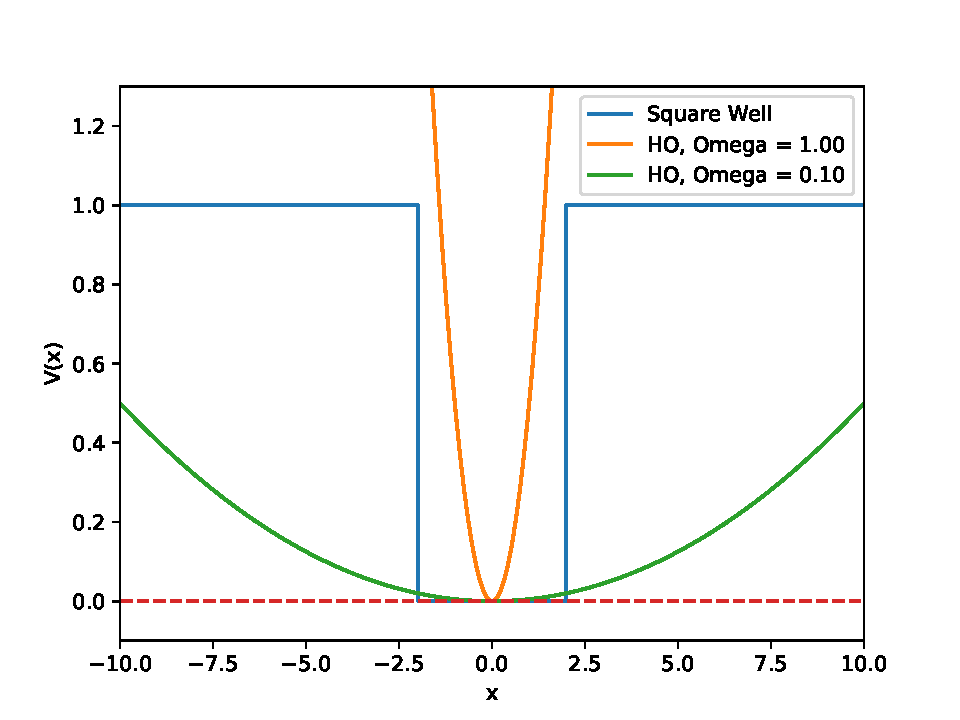
\includegraphics[width=\linewidth]{figures/SW_omega_comp}
\caption{Comparison between the finite square well potential and harmonic oscillators with different $\omega$ values. From the figure we can see the effect $\omega$ has on how good a fit harmonic oscillator basis functions are to the finite square well potential. It appears that the optimal $\omega$ value would be somewhere between $\omega = 0.1$ and $\omega = 1$.}
\label{fig: FSW_omega_comp}
\end{figure}

\subsubsection{Three Dimensions}

For the three-dimensional case we see from Table \ref{tab: EnergiesFSW3D} that we need a lot more basis function for the energies to converge than we did for the two-dimensional case. As always we expect the energies to be greater for three-dimensions than for two-dimensions, and from the table we see that that holds true here as well.

\begin{table}[!ht]
  \centering
  \begin{tabular}{c c c c c}
    \hline
    \hline
    $N$ & $\omega$ & Basis Functions & $E_\textrm{coeff}$ \\*
    \hline
    2 & 0.10 & 165 & 1.412(5) \\*
      & 0.10 & 364 & 1.411(5) \\*
      & 1.00 & 165 & 1.465(3) \\*
      & 1.00 & 364 & 1.463(3) \\*
    \hline
    \hline
  \end{tabular}
  \caption{The table lists ground state energy results for various finite square well systems in three dimensions. $N$ is the number of particles. $E_\textrm{coeff}$ are the energies obtained when the single particle wave functions are approximated by expansion in a single harmonic oscillator basis, and $\omega$ is the harmonic oscillator frequency used for the harmonic oscillator basis functions. The numbers in parenthesis are the statistical errors found using blocking. The amount of basis functions needed for the energies to converge is a lot greater for three dimensions than for two.}
  \label{tab: EnergiesFSW3D}
\end{table}

\subsection{One-Body Densities}

For the specific finite square well we have looked at in this thesis we expect all particles to be within the well, so-called bound particles, if the number of particles $N$ is $6$ or less. For our well being inside the well corresponds to having $r<\sqrt{8}$. Since the walls are $x,y = 2$ away from the center, the furthest away from the center a particle should be is in one of the corners, i.e. the particle would have $x$ and $y$ positions close to $\pm 2$, which would give an $r$ value close to $\sqrt{2^2 + 2^2}$. So for the one-body density we expect the distribution of $r$ to be $0$ at $r>\sqrt{8}$. 

From Figure \ref{fig:FSW_N2_2d} we see that for $N=2$, $\omega = 0.1$ and $15$ basis functions the particles are not completely bound, but for $\omega = 1$ they are (mostly). However, as the number of basis functions increase the distribution for $\omega = 0.1$ converges towards a final shape quicker than for $\omega = 1$. This fits with the energy results, where we saw that for $\omega = 0.1$ we need more basis functions to get good results, but for $\omega = 0.1$ we also find the optimal $\beta$ value with fewer basis functions. The shape for $\omega = 0.1$ is worse with $15$ basis functions because, even with an optimal $\beta$, $\omega = 0.1$ yields bad results for that few basis functions. However, the shape for $\omega = 0.1$ improves quicker as the number of basis functions increases because the optimal $\beta$ is reached with fewer basis functions. From Figure \ref{fig:FSW_N6_2d} we see that for $N=6$ with $\omega = 0.1$, the issue from $N=2$ with $15$ basis functions occurs even if we use $45$ basis functions. This shows the need for more basis functions as the number of particles increases.

Unlike for harmonic oscillator potential, for the square well potential the strength of the potential is constant until we hit one of the walls, at which point the potential skyrockets. For $N=2$ we should then expect the most likely position of the particle to be one that minimizes the repulsive forces between them while still keeping both particles within the well. In order to achieve this the particles should be in corners diagonally opposite of each other. This would mean that the distribution of $r$ should have a top at $r \approx \sqrt{8}$ in the two-dimensional case. However, when we look at our distributions in Figure \ref{fig:FSW_N2_2d_b} we see that the top of the distributions are typically between $r=1$ and $r=2$. This is likely due to the fact that we keep $\alpha$ constant at $1$, and doing a Hartree-Fock calculation on the overlap coefficient and properly optimizing $\alpha$ should solve this issue. From Figure \ref{fig:FSW_density3D} we can see that for $N=6$ particles the distribution has tops in the four corners, which is expected since it suggests that it is most likely for there to be one particle in each corner, and the last two being somewhere in the middle.

\begin{figure}[!ht]
\centering
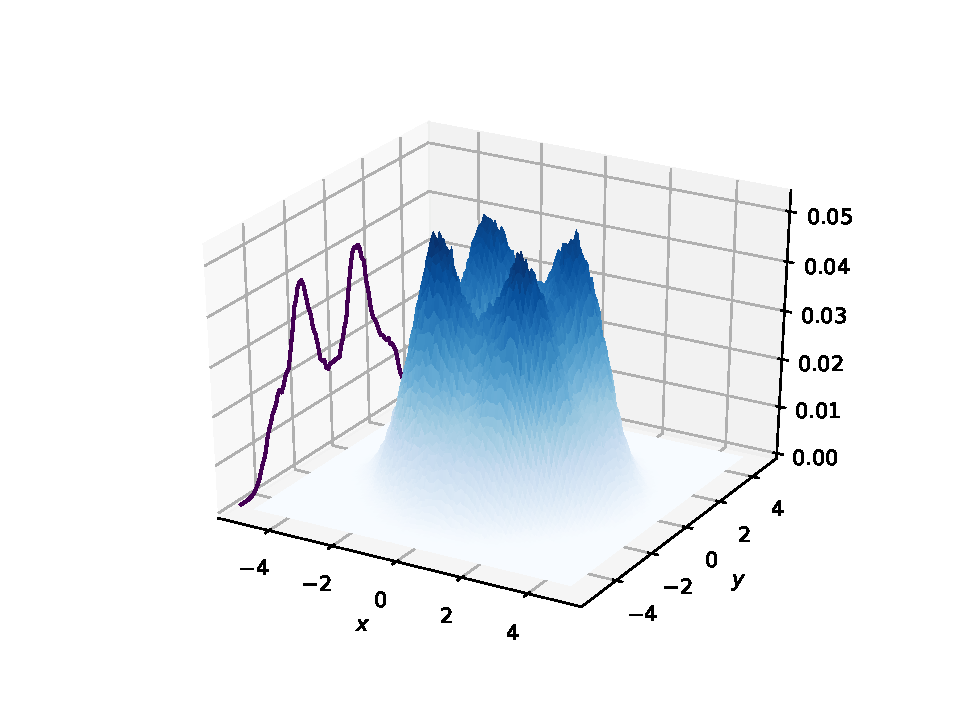
\includegraphics[width=\linewidth]{figures/densityFSW/density3D_FSW_N6_Omega1_2d_BF45}
\caption{The figures show the distributions of positions for a mesh-grid of the $x$ and $y$ positions for a finite square well potential. The number of particles is $N$ and the harmonic oscillator frequency used for the basis functions is $\omega=1$. We see that the distribution has tops at the corners of the well, which makes sense since the strength of the potential is equal everywhere inside the well and the Coulomb repulsion pushes the particles away from each other.} \label{fig:FSW_density3D}
\end{figure}

\begin{figure}
\centering
\begin{subfigure}{0.48\textwidth}
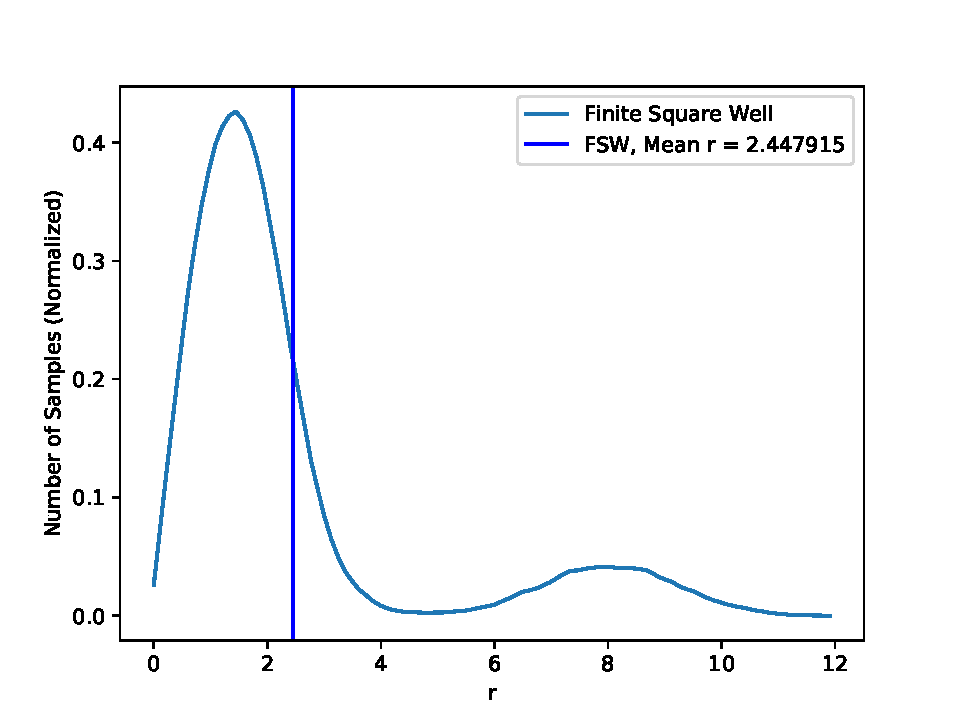
\includegraphics[width=\linewidth]{figures/densityFSW/density_FSW_N2_Omega010_2d_BF15.pdf}
\caption{$\omega=0.1$, $15$ Basis Functions} \label{fig:FSW_N2_2d_a}
\end{subfigure}\hspace*{\fill}
\begin{subfigure}{0.48\textwidth}
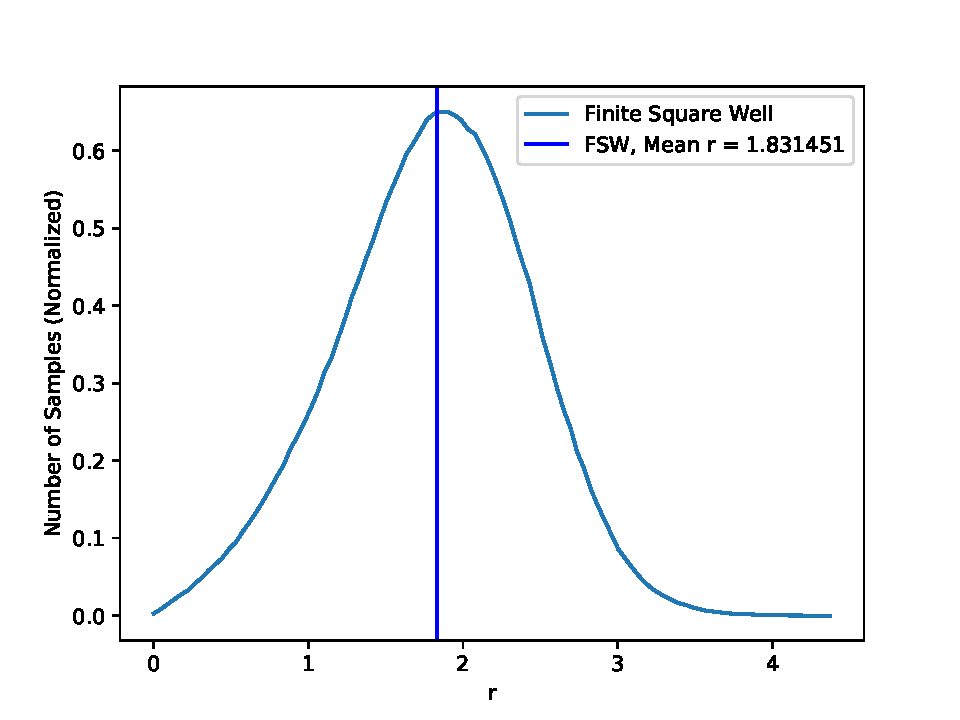
\includegraphics[width=\linewidth]{figures/densityFSW/density_FSW_N2_Omega1_2d_BF15.pdf}
\caption{$\omega=1$, $15$ Basis Functions} \label{fig:FSW_N2_2d_b}
\end{subfigure}

\medskip
\begin{subfigure}{0.48\textwidth}
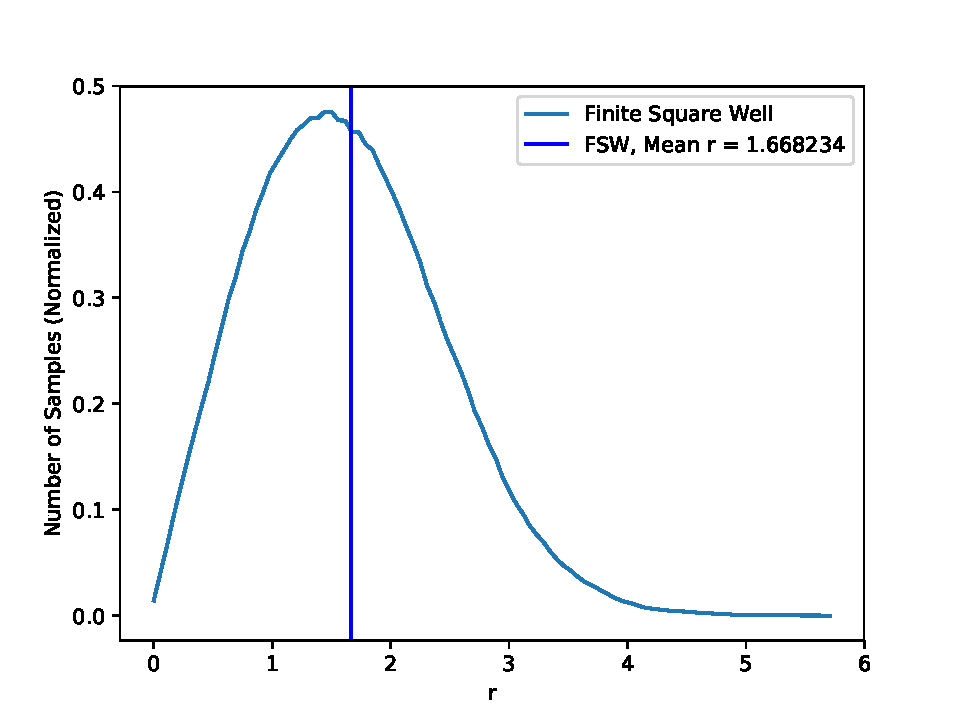
\includegraphics[width=\linewidth]{figures/densityFSW/density_FSW_N2_Omega010_2d_BF45.pdf}
\caption{$\omega=0.1$, $45$ Basis Functions} \label{fig:FSW_N2_2d_c}
\end{subfigure}\hspace*{\fill}
\begin{subfigure}{0.48\textwidth}
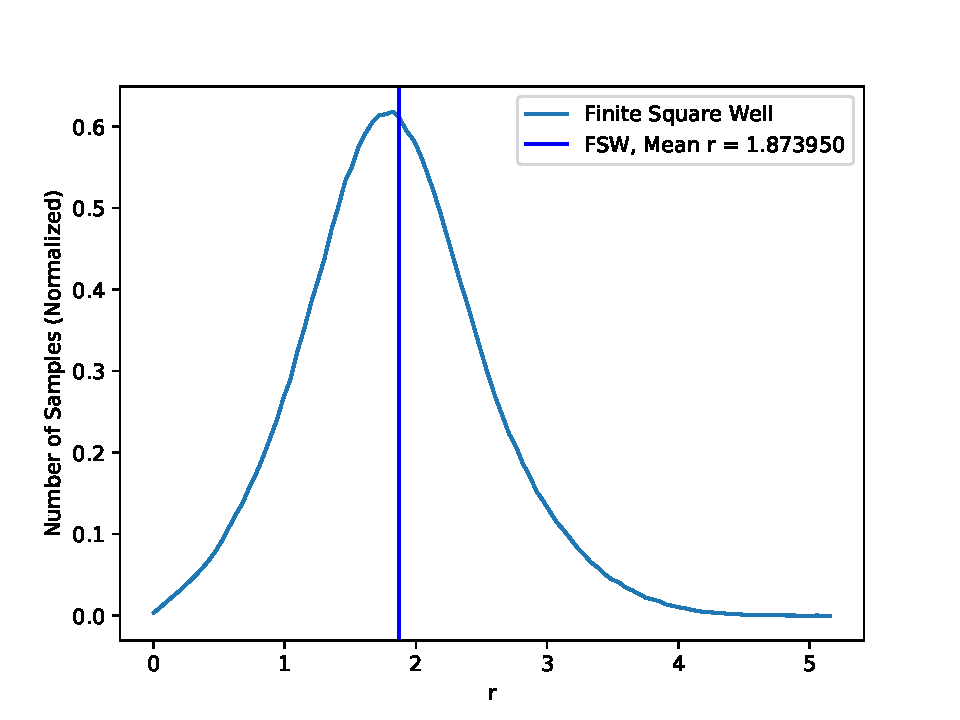
\includegraphics[width=\linewidth]{figures/densityFSW/density_FSW_N2_Omega1_2d_BF45.pdf}
\caption{$\omega=1$, $45$ Basis Functions} \label{fig:FSW_N2_2d_d}
\end{subfigure}

\medskip
\begin{subfigure}{0.48\textwidth}
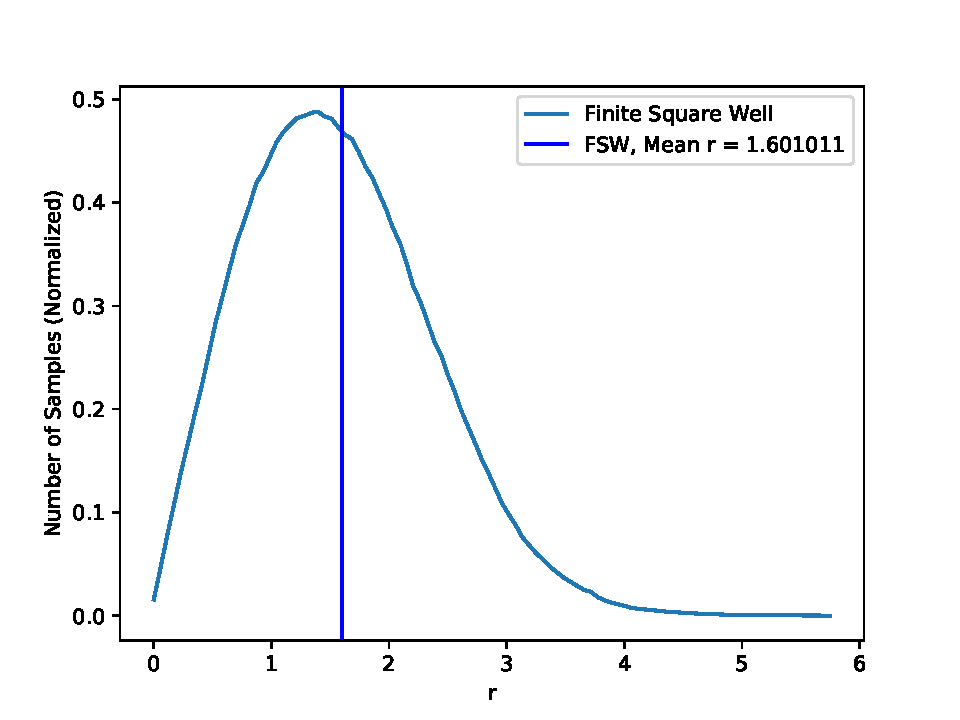
\includegraphics[width=\linewidth]{figures/densityFSW/density_FSW_N2_Omega010_2d_BF120.pdf}
\caption{$\omega=0.1$, $120$ Basis Functions} \label{fig:FSW_N2_2d_e}
\end{subfigure}\hspace*{\fill}
\begin{subfigure}{0.48\textwidth}
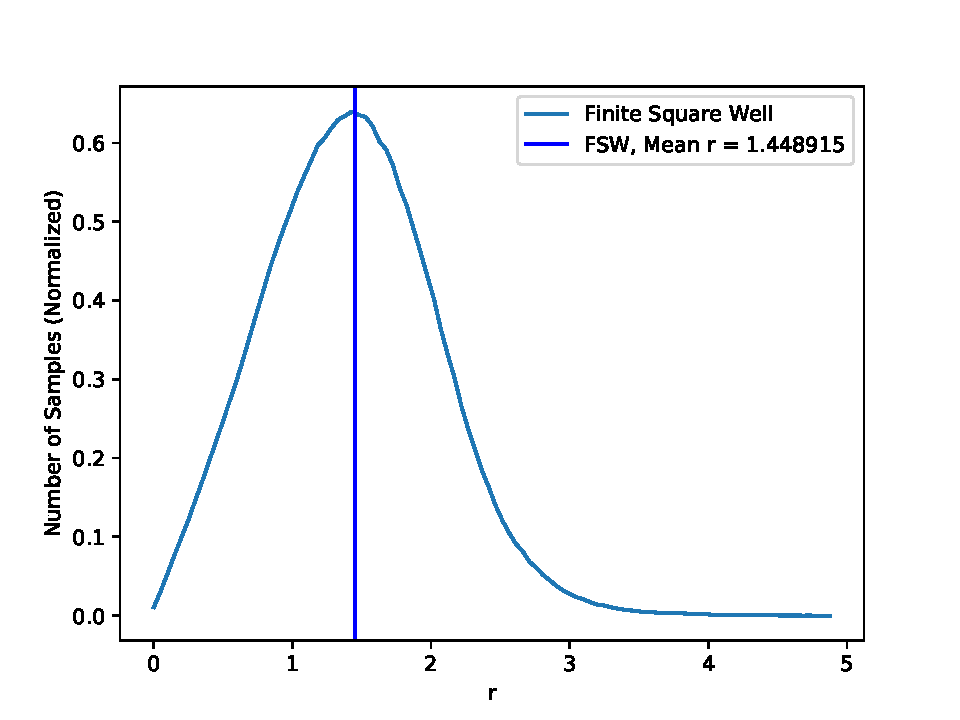
\includegraphics[width=\linewidth]{figures/densityFSW/density_FSW_N2_Omega1_2d_BF120.pdf}
\caption{$\omega=1$, $120$ Basis Functions} \label{fig:FSW_N2_2d_f}
\end{subfigure}

\caption{One-body densities for a two-dimensional finite square well potential with $N=2$ particles. The distance between the well center and each wall is $2$, and the potential is $0$ inside the well and $1$ outside.} \label{fig:FSW_N2_2d}
\end{figure}


\begin{figure}
\centering
\begin{subfigure}{0.48\textwidth}
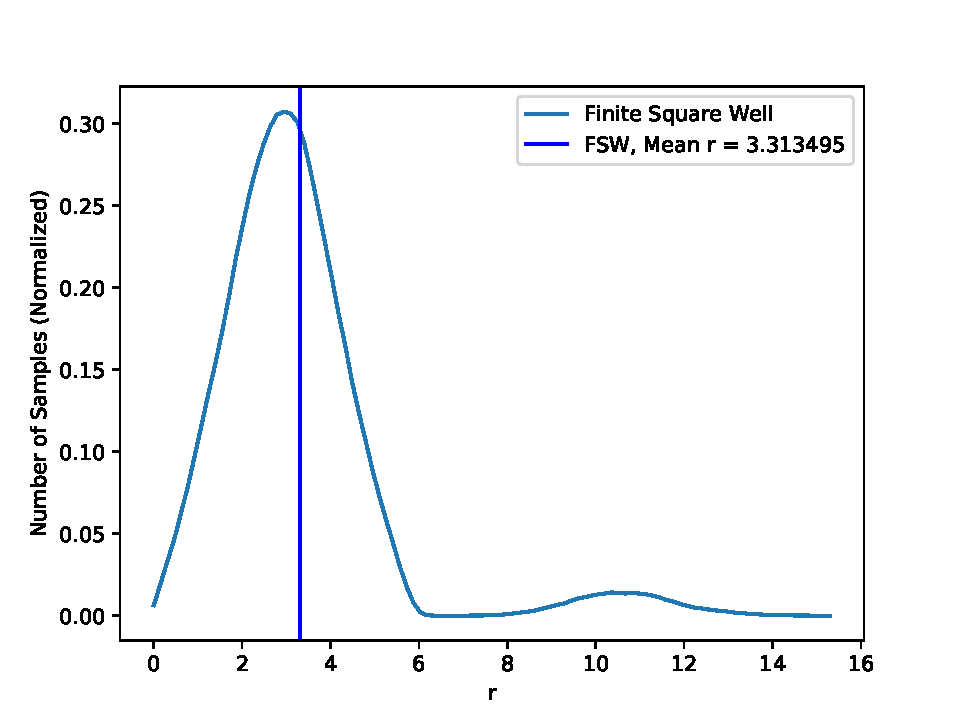
\includegraphics[width=\linewidth]{figures/densityFSW/density_FSW_N6_Omega010_2d_BF45.pdf}
\caption{$\omega=0.1$, $45$ Basis Functions} \label{fig:FSW_N6_2d_a}
\end{subfigure}\hspace*{\fill}
\begin{subfigure}{0.48\textwidth}
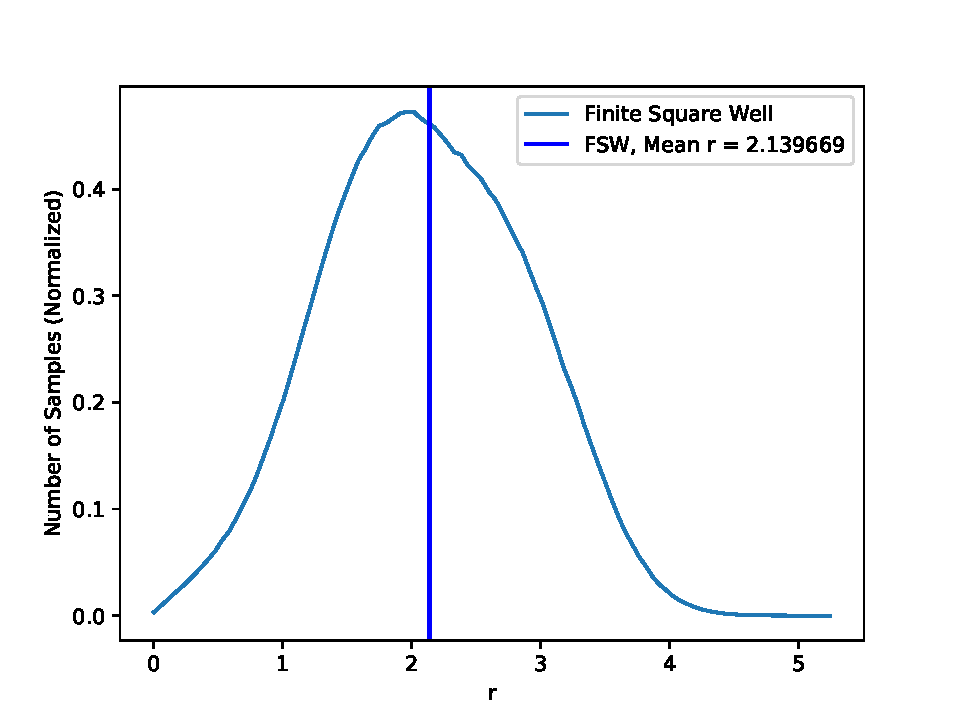
\includegraphics[width=\linewidth]{figures/densityFSW/density_FSW_N6_Omega1_2d_BF45.pdf}
\caption{$\omega=1$, $45$ Basis Functions} \label{fig:FSW_N6_2d_b}
\end{subfigure}

\caption{One-body densities for a two-dimensional finite square well potential with $N=6$ particles. The distance between the well center and each wall is $2$, and the potential is $0$ inside the well and $1$ outside.} \label{fig:FSW_N6_2d}
\end{figure}


\begin{figure}
\centering
\begin{subfigure}{0.48\textwidth}
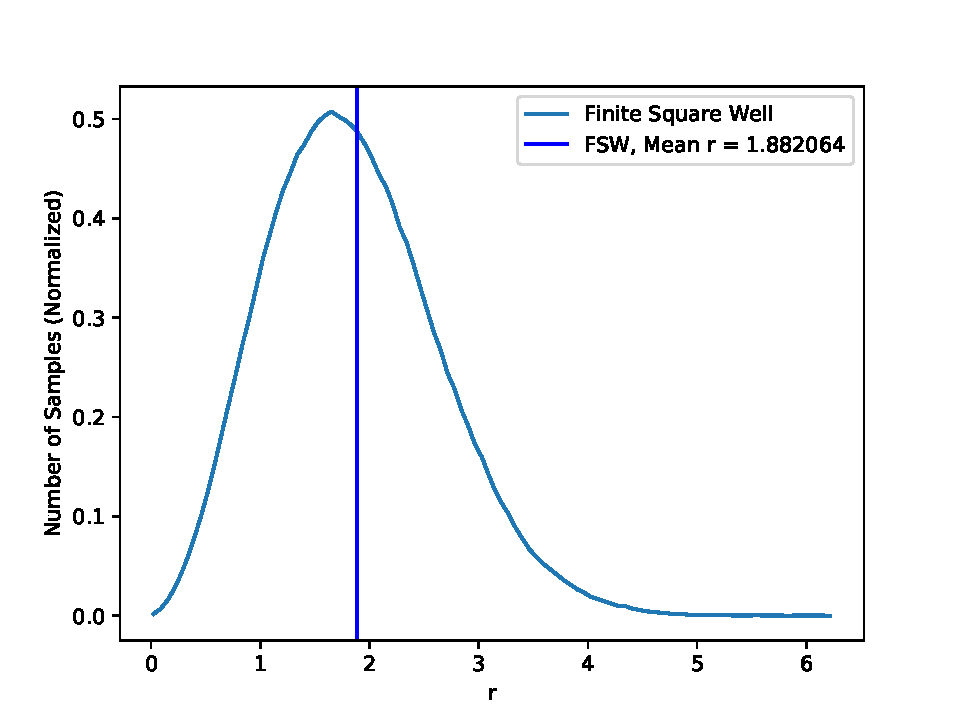
\includegraphics[width=\linewidth]{figures/densityFSW/density_FSW_N2_Omega010_3d_BF364.pdf}
\caption{$\omega=0.1$, $364$ Basis Functions} \label{fig:FSW_N2_3d_a}
\end{subfigure}\hspace*{\fill}
\begin{subfigure}{0.48\textwidth}
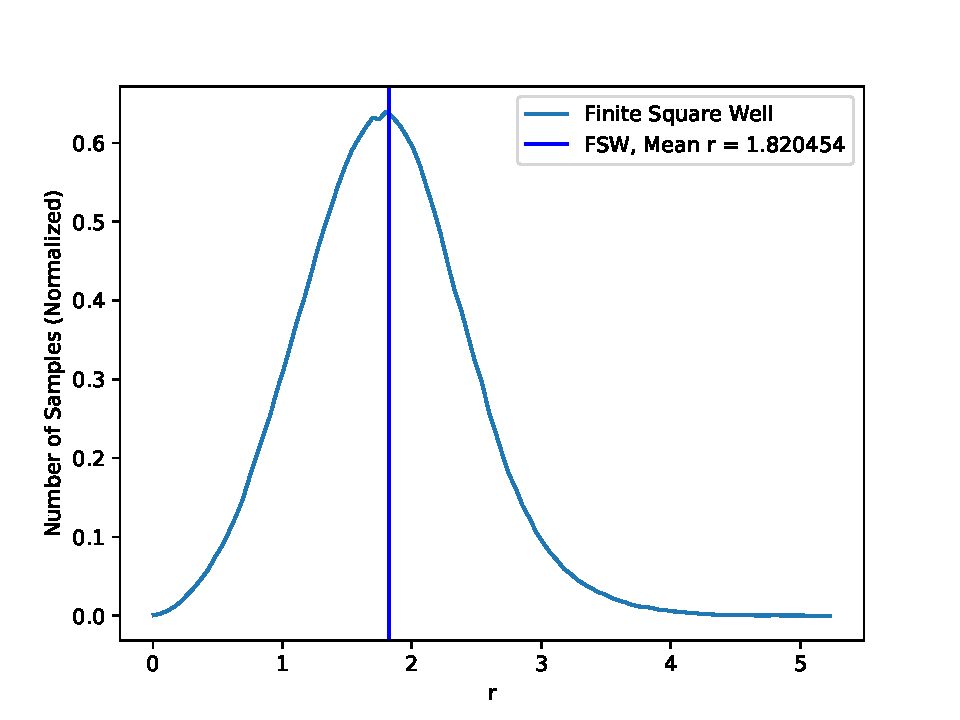
\includegraphics[width=\linewidth]{figures/densityFSW/density_FSW_N2_Omega1_3d_BF364.pdf}
\caption{$\omega=1$, $364$ Basis Functions} \label{fig:FSW_N2_3d_b}
\end{subfigure}

\caption{One-body densities for a three-dimensional finite square well potential with $N=2$ particles. The distance between the well center and each wall is $2$, and the potential is $0$ inside the well and $1$ outside.} \label{fig:FSW_N2_3d}
\end{figure}

\begin{comment}
\section{Wave Function Expanded in Harmonic Oscillator Basis}
\begin{table}[!ht]
  \centering
  \begin{tabular}{ | c | c | c | }
    \hline
    $N$ & $E$ (\textrm{Shared start}) & $E$ (\textrm{Split start}) \\*
    \hline
    $2$ & $2.00002$ & $2.00002$ \\*
    \hline
    $4$ & $4.00005$ & $4.00005$ \\*
    \hline
    $6$ & $8.00009$ & $8.0001$ \\*
    \hline
  \end{tabular}
  \caption{Unperturbed energies for the double well when approximating the single particle wave functions with harmonic oscillator basis functions. Results in the second column are for when all the particles starts in the same well and are then distributed between the wells by the program, while the results in the third column are for when we force half of the particles in each well at the start. Two dimensional system, $L_x=4$, $\omega=1$.}
  \label{tab: unperturbedEnergiesCoeff}
\end{table}

\begin{table}[!ht]
  \centering
  \begin{tabular}{ | c | c | c | }
    \hline
    $N$ & $E$ (\textrm{Shared start}) & $E$ (\textrm{Split start}) \\*
    \hline
    $2$ & $3.00854$ & $2.34952$ \\*
    \hline
    $4$ & $6.53324$ & $6.53747$ \\*
    \hline
    $6$ & $14.1804$ & $14.2108$ \\*
    \hline
  \end{tabular}
  \caption{Perturbed energies for the double well when approximating the single particle wave functions with harmonic oscillator basis functions. Results in the second column are for when all the particles starts in the same well and are then distributed between the wells by the program, while the results in the third column are for when we force half of the particles in each well at the start. Two dimensional system, $L_x=4$, $\omega=1$.}
  \label{tab: perturbedEnergiesCoeff}
\end{table}

\section{Wave Function as Super Postion of two Harmonic Oscillator Functions}
\begin{table}[!ht]
  \centering
  \begin{tabular}{ | c | c | c | }
    \hline
    $N$ & $E$ (\textrm{Shared start}) & $E$ (\textrm{Split start}) \\*
    \hline
    $2$ & $2$ & $2$ \\*
    \hline
    $4$ & $4$ & $4$ \\*
    \hline
    $6$ & $8$ & $8$ \\*
    \hline
  \end{tabular}
  \caption{Unperturbed energies for the double well when approximating the single particle wave functions with a super position of two harmonic oscillator functions. Results in the second column are for when all the particles starts in the same well and are then distributed between the wells by the program, while the results in the third column are for when we force half of the particles in each well at the start. Two dimensional system, $L_x=4$, $\omega=1$.}
  \label{tab: unperturbedEnergiesSupPos}
\end{table}

\begin{table}[!ht]
  \centering
  \begin{tabular}{ | c | c | c | }
    \hline
    $N$ & $E$ (\textrm{Shared start}) & $E$ (\textrm{Split start}) \\*
    \hline
    $2$ & $3.00852$ & $2.3495$ \\*
    \hline
    $4$ & $6.53322$ & $6.53742$ \\*
    \hline
    $6$ & $14.4748$ & $13.872$ \\*
    \hline
  \end{tabular}
  \caption{Perturbed energies for the double well when approximating the single particle wave functions with a super position of two harmonic oscillator functions. Results in the second column are for when all the particles starts in the same well and are then distributed between the wells by the program, while the results in the third column are for when we force half of the particles in each well at the start. Two dimensional system, $L_x=4$, $\omega=1$.}
  \label{tab: perturbedEnergiesSupPos}
\end{table}
\end{comment}

\end{document}